\chapter{递质释放} \label{chap:chap15}

大脑的一些最显著的能力(例如学习和记忆)被认为源于化学突触的基本特性,其中突触前细胞释放化学递质,激活突触后细胞膜中的受体。
在大多数中央突触中,递质从突触前细胞的突触前细胞释放,突触前末梢沿着轴突(就像串再绳子上的珠子)膨胀,膨胀中充满了突触小泡和其他与突触后靶点接触的细胞器。
在其他突触,包括神经肌肉接头处,递质从轴突末梢的突触前末梢释放。
为方便起见,我们将这 2 种类型的释放位点称为突触前末梢。
在最后的第~\ref{chap:chap14}-\ref{chap:chap16}章中,我们了解了突触后受体如何控制产生突触后电位的离子通道。
在这里,我们考虑突触前末梢的电事件和生化事件如何导致小分子神经递质的快速释放,例如\textit{乙酰胆碱}、谷氨酸和 \textit{$\gamma$-氨基丁酸},它们是快速突触传递的基础。
在下一章中,我们将研究神经递质本身以及生物胺(\textit{5-羟色氨}、去甲肾上腺素和多巴胺)和神经肽的化学性质,它们是细胞间信号传导较慢形式的基础。



\section{递质释放受突触前末梢去极化调控}

突触前末梢的什么事件导致了递质释放?
\textit{伯纳德$\cdot$卡茨}和\textit{里卡多$\cdot$米里迪}首先证明了突触前膜去极化的重要性。
为此,他们使用了鱿鱼的巨大突触,这种突触大到足以让电极插入突触前和突触后结构。
如图~\ref{fig:15_1}A~所示,2 个电极插入突触前末梢(一个用于刺激,一个用于记录),一个电极插入突触后细胞用于记录\textit{兴奋性突触后电位},它提供了递质释放的指标。


\begin{figure}[htbp]
	\centering
	\includegraphics[width=0.9\linewidth]{chap15/fig_15_1}
	\caption{递质释放由突触前膜电位的变化触发\cite{katz1967study}。
	A. 电压记录电极插入鱿鱼星状神经节中巨型突触的突触前纤维和突触后纤维。
	电流通过电极也插入突触前引发了突触前动作电位。
	B. 将\textit{河豚毒素}添加到侵泡细胞的溶液中,以阻断作为动作电位基础的电压门控~\ce{Na+} 通道。
	随着越来越多的~\ce{Na+}通道被阻断,突触前动作电位和\textit{兴奋性突触后电位}的振幅逐渐降低。
	7 分钟后,突触前动作电位仍可产生超阈值的\textit{兴奋性突触后电位},触发突触后细胞的动作电位。
	大约 14 到 15 分钟后,突触前脉冲逐渐变小并产生较小的突触后去极化。
	当突触前峰值降低到 40 毫伏或更低时,它无法产生\textit{兴奋性突触后电位}。
	因此,突触前去极化的大小(此处由动作电位提供)控制递质释放的幅度。
	C. \textit{兴奋性突触后电位}振幅对突触前动作电位振幅的依赖性是递质释放输入-输出曲线的基础。
	这种关系是通过在\textit{河豚毒素}阻断突触前\ce{Na+}通道开始期间刺激突触前神经获得的,此时突触前动作电位和突触后去极化的幅度逐渐降低。
	上图表明产生突触后电位需要 40 毫伏的突触前动作电位。
	超过这个阈值,\textit{兴奋性突触后电位}的振幅会急剧增加,以响应突触前电位振幅的小幅增加。
	突触前脉冲和\textit{兴奋性突触后电位}之间的关系是对数关系,如下图所示。
	突触前脉冲增加 13.5 毫伏会使\textit{兴奋性突触后电位}增加 10 倍。}
	\label{fig:15_1}
\end{figure}
突触前神经元受到刺激并发出动作电位后,突触后细胞中会记录下足以触发动作电位的\textit{兴奋性突触后电位}。
\textit{卡兹}和\textit{米里}随后研究了突触前动作电位如何触发递质释放。
他们发现,当电压门控 \ce{Na+} 通道被河豚毒素阻断时,连续动作电位会逐渐变小。
如图~\ref{fig:15_1}B~所示,随着动作电位的减小,\textit{兴奋性突触后电位}相应减小。
当 \ce{Na+} 通道阻滞变得如此严重以至于将突触前脉冲的振幅降低到 40 毫伏以下(相对于静息电位为正)时,\textit{兴奋性突触后电位}将完全消失。
因此,如图~\ref{fig:15_1}C~所示,递质释放量(通过突触后去极化的大小测量)是突触前去极化量的\textit{阶梯函数}。


\textit{卡兹}和\textit{米里}接下来研究了突触前去极化如何触发递质释放。
动作电位由~\ce{Na+}流入和~\ce{K+}通过电压门控通道流出产生。
为了确定触发递质释放是否需要~\ce{Na+}流入或~\ce{K+}流出,\textit{卡兹}和\textit{米里}首先用河豚毒素阻断了~\ce{Na+}通道。
然后他们研究通过电流注入对突触前膜的直接去极化是否仍会触发递质释放。
事实上,突触前膜的去极化超过约 40 毫伏的阈值(相对于静息电位为正)会在突触后细胞中引发\textit{兴奋性突触后电位}(即使~\ce{Na+}通道被阻断)。
超过该阈值,逐渐增加的去极化会导致逐渐增加的递质释放量。
如图~\ref{fig:15_2}B~所示,该结果表明突触前~\ce{Na+}流入不是释放所必需的;
它的重要性仅在于它使膜去极化因此发生递质释放。


\begin{figure}[htbp]
	\centering
	\includegraphics[width=1.0\linewidth]{chap15/fig_15_2}
	\caption{递质释放不是由突触前电压门控~\ce{Na+}或~\ce{K+} 通道的打开直接触发的\cite{katz1967study}。
	A. 电压记录电极插入鱿鱼星状神经节中巨型突触的突触前纤维和突触后纤维。
	电流通过电极也插入突触前细胞。
	B. 通过微电极直接注入电流使突触前末梢去极化,即使通过向细胞沐浴液中添加\textit{河豚毒素}完全阻断电压门控\ce{Na+}通道后,也可以触发递质释放。
	3 组迹线表示(从下到上)注入突触前末梢的去极化电流脉冲(I)、突触前末梢产生的电位(Pre)以及递质释放到突触后细胞上产生的\textit{兴奋性突触后电位}。
	突触前细胞中逐渐增强的电流脉冲会相应地产生更大的突触前末梢去极化。
	突触前去极化越大,\textit{兴奋性突触后电位}越大。
	突触前去极化不会在去极化电流脉冲的整个持续时间内保持,因为电压门控 \ce{K+} 通道的延迟激活会导致复极化。
	C. 即使在电压门控 \ce{Na+} 通道已被\textit{河豚毒素}阻断并且电压门控 \ce{K+} 通道已被\textit{四乙铵}阻断后,也会发生递质释放。
	在这个实验中,\textit{四乙铵}被注入突触前末梢。
	这 3 组轨迹代表与 B 部分相同的测量值。
	由于突触前 \ce{K+} 通道被阻断,因此在整个电流脉冲中保持突触前去极化。
	大量持续的突触前去极化产生大量持续的\textit{兴奋性突触后电位}。
	D. 阻断\ce{Na+}和\ce{K+}通道可以准确控制突触前电压并确定完整的输入-输出曲线。
	超过某个阈值(相对于静息电位为 40 毫伏正值),从\textit{兴奋性突触后电位}的大小测量,突触前去极化和递质释放之间存在陡峭的关系。
	大于一定水平的去极化不会导致递质的任何额外释放。
	最初的突触前静息膜电位约为 -70 毫伏。}
	\label{fig:15_2}
\end{figure}


为了检查 \ce{K+} 流出对递质释放的贡献,\textit{卡兹}和\textit{米里}在用河豚毒素阻断电压敏感~\ce{Na+}通道的同时,用四乙铵阻断了电压门控 \ce{K+} 通道。
如图~\ref{fig:15_2}C~所示,然后他们将去极化电流注入突触前末梢,发现\textit{兴奋性突触后电位}大小正常,表明发生了正常的递质释放。
因此,递质释放不需要 \ce{Na+} 和 \ce{K+} 通量。


在存在四乙铵的情况下,电流脉冲在整个脉冲持续时间内引起突触前去极化,因为通常使突触前膜复极化的 \ce{K+} 电流被阻断。
因此,如图~\ref{fig:15_2}C~所示,递质释放在整个电流脉冲中持续存在,这反映在突触后细胞的长期去极化中。
如图~\ref{fig:15_2}D~所示,\textit{卡兹}和\textit{米里}使用持续去极化的量化来确定将突触前去极化与递质释放相关的完整输入-输出曲线。
他们证实了递质释放对突触前去极化的严重依赖。
在递质释放增加的去极化范围内(40-70 毫伏正向静息水平),突触前去极化增加 10 毫伏会使递质释放增加 10 倍。
超过上限的突触前膜去极化不会进一步增加突触后电位。



\section{\ce{Ca^2+} 内流激发释放}

\textit{卡兹}和\textit{米里}接下来将注意力转向了 \ce{Ca^2+}。
早些时候,\textit{卡兹}和\textit{卡斯蒂略}发现增加细胞外 \ce{Ca^2+} 浓度会增强递质释放,而降低浓度会减少并最终阻断突触传递。
因为递质释放是一个细胞内过程,这些发现暗示 \ce{Ca^2+} 必须进入细胞才能影响递质释放。


先前对鱿鱼巨型轴突膜的研究已经确定了一类电压门控 \ce{Ca^2+} 通道,由于对 \ce{Ca^2+} 的内向电化学驱动力大,因此打开该通道会导致大量 \ce{Ca^2+} 流入。
细胞外 \ce{Ca^2+} 浓度,在脊椎动物中约为 2 毫摩尔,通常比细胞内浓度高 4 个数量级,在静止时约为 $10^{-7}$ 摩尔。
然而,由于这些 \ce{Ca^2+} 通道沿轴突分布稀疏,它们本身无法提供足够的电流来产生再生动作电位。


\textit{卡兹}和\textit{米里}发现 \ce{Ca^2+} 通道在突触前末梢更为丰富。
在那里,在\textit{四乙铵}和\textit{河豚毒素}存在的情况下,去极化电流脉冲有时能够触发再生去极化,这需要细胞外 \ce{Ca^2+},即钙脉冲。
\textit{卡兹}和\textit{米里}因此提出 \ce{Ca^2+} 具有双重功能。
它是动作电位期间去极化电荷的载体(如 \ce{Na+}),并且是一种特殊的化学信号(第二信使),将有关膜电位变化的信息传递给负责递质释放的细胞内机制。
\ce{Ca^2+} 能够作为一种有效的化学信号,因为它们的细胞内静息浓度较低,比 \ce{Na+} 的静息浓度低约 105 倍。
因此,在动作电位期间进入或离开细胞的少量 \ce{Ca^2+} 会导致细胞内 \ce{Ca^2+} 发生较大百分比的变化,从而引发各种生化反应。
最近的实验证明了 \ce{Ca^2+} 通道在释放中的重要性,这些实验表明阻断 \ce{Ca^2+} 通道的特定毒素也会阻断释放。


\textit{鲁道夫$\cdot$利纳斯}和他的同事测量了鱿鱼突触前末梢的电压门控 \ce{Ca^2+} 通道的特性。
\textit{利纳斯}使用电压钳使末梢去极化,同时用河豚毒素阻断电压门控 \ce{Na+} 通道,用四乙基铵阻断 \ce{K+} 通道。
如图~\ref{fig:15_3}~所示,他发现分级去极化激活分级内向 \ce{Ca^2+} 电流,这反过来导致递质分级释放。
\ce{Ca^2+} 电流分级,因为 \ce{Ca^2+} 通道与电压门控 \ce{Na+} 和 \ce{K+} 通道一样具有电压门控。
然而,乌贼末梢的 \ce{Ca^2+} 通道与 \ce{Na+} 通道不同,因为它们不会迅速失活,而是在突触前去极化持续期间保持开放。


\begin{figure}[htbp]
	\centering
	\includegraphics[width=0.7\linewidth]{chap15/fig_15_3}
	\caption{递质释放受 \ce{Ca^2+} 通过电压门控 \ce{Ca^2+} 通道流入突触前末梢的调节。
	乌贼巨型突触中电压敏感的 \ce{Na+} 和 \ce{K+} 通道被河豚毒素和四乙铵阻断。
	突触前末梢的膜被电压钳位,膜电位步进到 6 个不同的去极化指令水平(底部)。
	突触后去极化的幅度(上)随突触前内向 \ce{Ca^2+} 电流(中)的大小而变化,因为递质释放量是突触前末梢 \ce{Ca^2+} 浓度的函数。
	突触后电位轨迹中的缺口是关闭突触前命令电位的结果\cite{llinas1977depolarization}。}
	\label{fig:15_3}
\end{figure}


如图~\ref{fig:15_4}~所示,\ce{Ca^2+}通道主要位于活动区的突触前末梢,神经递质释放的位置,正好与突触后受体相对。
这种定位很重要,因为 \ce{Ca^2+} 不会从其进入位点扩散很远的距离,因为游离 \ce{Ca^2+} 会被 \ce{Ca^2+} 结合蛋白快速缓冲。
结果,\ce{Ca^2+} 流入导致活性区的 \ce{Ca^2+} 浓度局部急剧上升。 
如图~\ref{fig:15_4}B~所示,使用 \ce{Ca^2+} 敏感性荧光染料可以观察到突触前末梢 \ce{Ca^2+} 的增加。
所有突触处递质释放的一个显著特征是它对 \ce{Ca^2+} 流入的急剧非线性依赖性;
\ce{Ca^2+} 内流增加 2 倍可使递质释放量增加 16 倍以上。 
这种关系表明,在某些调节位点,\ce{Ca^2+}传感器需要多个 \ce{Ca^2+} 的协同结合才能触发释放。


\begin{figure}[htbp]
	\centering
	\includegraphics[width=1.0\linewidth]{chap15/fig_15_4}
	\caption{在神经肌肉接头的突触传递过程中流入突触前神经末梢的~\ce{Ca^2+}集中在活动区。
	终板突触前末梢的~\ce{Ca^2+}通道集中在突触后肌膜上烟碱\textit{乙酰胆碱}受体簇的对面。
	两幅图展示了青蛙的神经肌肉接头。
	A. 放大图显示了神经肌肉接头的显微解剖结构,突触前末梢被剥离。
	荧光图像显示了突触前 \ce{Ca^2+} 通道(标记有与 \ce{Ca^2+} 通道结合的德克萨斯红偶联的海洋蜗牛毒素)和突触后\textit{乙酰胆碱}受体(标记有荧光标记的 $\alpha$-金环蛇毒素,它选择性地结合\textit{乙酰胆碱}受体)。
	这 2 个图像通常叠加在一起,但为了清晰起见已分开。
	2 种探针的标记模式几乎精确对齐,表明突触前神经元的活动区与含有高浓度\textit{乙酰胆碱}受体的突触后膜几乎完美对齐\cite{robitaille1990strategic}。
	B. 突触前末梢的钙流入位于活动区。
	钙可以使用 \ce{Ca^2+} 敏感的荧光染料进行可视化。
	1. 黑白图像显示了静息条件下充满 fura-2 (细胞内 \ce{Ca^2+}的特异性荧光指示剂)的神经肌肉接头处的突触前末梢。
	% fura-2百科:https://baike.baidu.com/item/fura-2/655995
	染料的荧光强度随着它与 \ce{Ca^2+} 的结合而变化。
	在彩色图像中,颜色编码的荧光强度变化显示细胞内 \ce{Ca^2+} 响应单个突触前动作电位的局部热点。
	红色表示 \ce{Ca^2+} 大量增加的区域;
	蓝色表示 \ce{Ca^2+} 几乎没有增加的区域。
	沿末梢可以看到 \ce{Ca^2+} 浓度的规则峰值,对应于 \ce{Ca^2+} 通道在活性区的定位。
	2. 彩色图像显示了末梢 \ce{Ca^2+} 水平峰值增加的高倍放大视图。
	相应的黑白图像显示了突触后膜中烟碱\textit{乙酰胆碱}受体的荧光标记,说明了突触前 \ce{Ca^2+} 流入区域与突触后受体区域之间的紧密空间对应关系\cite{wachman2004spatial}。}
	\label{fig:15_4}
\end{figure}



\subsection{突触前~\ce{Ca^2+}浓度与释放的关系}

诱导神经递质释放需要多少 \ce{Ca^2+}? 
为了解决这个问题,\textit{伯特$\cdot$萨克曼}和\textit{厄温$\cdot$内尔}及其同事测量了\textit{花萼突触}中的突触传递,\textit{花萼突触}是哺乳动物听觉脑干中的一个大突触,由从耳蜗核到\textit{斜方体}内侧核的轴突组成。
这个突触专门用于非常快速和可靠的传输,以允许在环境中精确定位声音。


如图~\ref{fig:15_5}A~所示,花萼形成一个杯状的突触前末梢,吞没了一个突触后细胞体。
花萼突触包括近千个作为独立释放位点的活动区。
这使得突触前动作电位能够释放大量递质,从而导致可靠的大突触后去极化。
相比之下,大脑中典型神经元的单个突触按钮仅包含一个活动区。
因为花萼末梢很大,所以可以将电极插入突触前和突触后结构,就像乌贼巨型突触一样,并直接测量 2 个隔间之间的突触耦合。
如图~\ref{fig:15_5}B~所示,这种配对记录可以精确确定突触前和突触后细胞活动的时间过程。


\begin{figure}[htbp]
	\centering
	\includegraphics[width=1.0\linewidth]{chap15/fig_15_5}
	\caption{已经测量了突触前 \ce{Ca^2+} 与中央突触中递质释放之间的精确关系\cite{meinrenken2003hodgkin,sun2007dual}。
	A. 哺乳动物中\textit{花萼突触}的大突触前末梢,脑干吞没突触后细胞体。
	左侧的荧光图像显示了一个充满 \ce{Ca^2+} 敏感染料的花萼。
	B. 几个突触事件的时间进程。
	虚线表示 \ce{Ca^2+} 电流、递质释放和突触后电流的峰值响应时间。
	C. 递质释放高度依赖于突触前末梢的 \ce{Ca^2+} 浓度。
	花萼装有笼状 \ce{Ca^2+} 化合物,该化合物可响应紫外线闪光释放其结合的 \ce{Ca^2+},并装有 \ce{Ca^2+} 敏感染料,可测量细胞内 \ce{Ca^2+} 浓度。
	通过控制光的强度,可以调节突触前末梢 \ce{Ca^2+} 的增加。
	该图以对数标度显示囊泡释放速率与细胞内 \ce{Ca^2+} 浓度之间的关系。
	蓝线描绘了一个模型的数据拟合,该模型假定释放是由结合 5 个 \ce{Ca^2+} 的主要 \ce{Ca^2+} 传感器触发的,导致 \ce{Ca^2+} 协同性为 5。
	由于 \ce{Ca^2+} 和释放之间的非线性关系,浓度超过 1 微摩尔时 \ce{Ca^2+} 的小增量会导致释放大量增加。
	D. 从囊泡中释放递质需要 5 个 \ce{Ca^2+} 与 \ce{Ca^2+} 敏感突触囊泡蛋白结合。
	在图中,\ce{Ca^2+} 与单个囊泡上存在的 5 个受体结合;
	实际上,每个\textit{受体分子}结合多个 \ce{Ca^2+}。}
	\label{fig:15_5}
\end{figure}


这些记录显示突触前动作电位和\textit{兴奋性突触后电位}之间存在 1 到 2 毫秒的短暂滞后,这就是\textit{谢林顿}所说的突触延迟。
因为 \ce{Ca^2+} 通道比 \ce{Na+} 通道打开得更慢,并且内向 \ce{Ca^2+} 驱动力随着神经元复极化而增加,所以 \ce{Ca^2+} 直到膜开始复极化才开始全力进入突触前末梢。
令人惊讶的是,一旦 \ce{Ca^2+} 进入末梢,递质就会迅速释放,延迟只有几百微秒。
因此,突触延迟主要归因于打开 \ce{Ca^2+} 通道所需的时间。
\ce{Ca^2+} 作用的惊人速度表明,在 \ce{Ca^2+} 流入之前,释放过程中的生化机制必须已经处于准备就绪状态。 
这种快速动力学对于神经元信息处理至关重要,需要我们稍后考虑的优雅分子机制。


突触前动作电位通常只会使突触前 \ce{Ca^2+} 浓度短暂升高,因为 \ce{Ca^2+} 通道只打开很短的时间。 
此外,\ce{Ca^2+} 流入到活性区。
如图~\ref{fig:15_5}B~所示,这 2 个特性有助于形成集中的局部 \ce{Ca^2+} 脉冲,从而引起递质释放的爆发。
正如我们将在本章后面看到的那样,动作电位的持续时间调节了流入末梢的 \ce{Ca^2+} 量,从而调节递质释放量。


为了确定需要多少 \ce{Ca^2+} 才能触发释放,\textit{内尔}和\textit{萨克曼}研究小组在突触前末梢引入了一种与光敏化学笼复合的非活性形式的 \ce{Ca^2+}。
他们还在末梢上加载了\ce{Ca^2+}敏感荧光染料,以测定细胞内游离 \ce{Ca^2+} 浓度。
通过用闪光解笼 \ce{Ca^2+},它们可以通过均匀且可量化的 \ce{Ca^2+} 浓度增加来触发递质释放。
这些实验表明,\ce{Ca^2+} 浓度升高小于 1 微摩尔就足以诱导某些递质的释放,但需要大约 10 至 30 微摩尔 \ce{Ca^2+} 才能释放在动作电位期间通常观察到的量。
同样,如图~\ref{fig:15_5}C、D~所示,\ce{Ca^2+} 浓度和递质释放之间的关系是高度非线性的,与至少 4 个或 5 个 \ce{Ca^2+} 必须与 \ce{Ca^2+} 传感器结合才能触发释放的模型一致。



\subsection{几类~\ce{Ca^2+} 通道介导递质释放}

\ce{Ca^2+}通道存在于所有神经细胞和许多非神经元细胞中。
在骨骼肌和心肌细胞中,它们对兴奋-收缩偶联很重要;
在内分泌细胞中,它们调节激素的释放。
神经元包含 5 大类电压门控 \ce{Ca^2+} 通道:L 型、P/Q 型、N 型、R 型和 T 型,它们由不同但密切相关的基因编码,这些基因可分为基于氨基酸序列相似性的 3 个基因家族。
L 型通道由 Ca$_V$1 家族编码。
Ca$_V$2 家族的成员包括 P/Q- (Ca$_V$2.1)、N- (Ca$_V$2.2) 和 R 型(Ca$_V$2.3)通道。
最后,T 型通道由 Ca$_V$3 基因家族编码。 
每种通道类型都具有特定的生物物理学和药理学特性以及生理功能(表~\ref{tab:15_1})。


\begin{table}[htbp]
	\caption{神经元的电压门控\ce{Ca^2+}通道} \label{tab:15_1} \centering
	\begin{tabular}{lllllll}
		\toprule
		通道 & 别名 & \makecell[l]{\ce{Ca^2+}通\\道类型}  & 组织 & 阻滞剂 & 电压门控 & 功能\\
		\midrule
		Ca$_v$V1.1−1.4 & $\alpha_{1C,D,F,S}$ & L & \makecell[l]{肌肉、\\神经元} & 二氢吡啶类 & \makecell[l]{高阈值或\\高压激活} & \makecell[l]{收缩、缓慢和一些\\有限的快速释放} \\
		Ca$_v$2.1 & $\alpha_{1A}$ & P/Q & 神经元 & \makecell[l]{美洲蜘蛛毒素\\(蜘蛛毒液)} & \makecell[l]{高阈值或\\高压激活} & 快速释放 +++ \\
		Ca$_v$2.2 & $\alpha_{1B}$ & N & 神经元 & \makecell[l]{芋螺毒素(锥状\\蜗牛毒液)} & \makecell{高阈值或\\高压激活} & 快速释放+++ \\
		Ca$_v$2.3 & $\alpha_{1E}$ & R & 神经元 & \makecell[l]{SNX-482\\(狼蛛毒液)} & \makecell[l]{高阈值或\\高压激活} & 快速释放 +++ \\
		Ca$_v$3.1–3.3 & $\alpha_{1G,H,I}$ & T & \makecell[l]{肌肉、\\神经元} & \makecell[l]{Mibefradil\\(有限选择性)} & 低电压激活 & 起搏器激活 \\
		\bottomrule
	\end{tabular}
\end{table}


\ce{Ca^2+}通道是多聚体蛋白质,其独特的特性由其成孔 $\alpha$1 亚基决定。
如图~\ref{fig:8_10}~所示,$\alpha$1 亚基与电压门控 \ce{Na+} 通道的$\alpha$亚基同源,由具有 6 个跨膜区段的结构域的 4 个重复组成,其中包括 S4 电压传感器和孔衬里 P 区。
\ce{Ca^2+}通道还具有辅助亚基(称为 $\alpha$2、$\beta$、$\gamma$ 和 $\delta$),它们可以改变由 $\alpha$1 亚基形成的通道的特性。
不同类型的\ce{Ca^2+}通道在神经元中的亚细胞定位也不同。
N 型和 P/Q 型 \ce{Ca^2+} 通道主要存在于突触前末梢,而 L 型、R 型和 T 型通道主要存在于胞体和树突中。


4 种类型的电压门控 \ce{Ca^2+} 通道(L 型、P/Q 型、N 型和 R 型)通常需要相当强的去极化才能被激活(需要正至 −40 至 −20 毫伏的电压),因此有时被宽泛地称为高电压激活的 \ce{Ca^2+} 通道(表~\ref{tab:15_1})。
相反,T 型通道响应于产生动作电位(-60 至 -40 毫伏)阈值附近的小去极化而打开,因此被称为低电压激活的 \ce{Ca^2+} 通道。
因为它们被膜电位的微小变化激活,所以 T 型通道有助于控制静息电位的兴奋性,并且是驱动大脑和心脏中某些细胞节律性起搏器活动的兴奋性电流的重要来源。


在神经元中,快速突触传递过程中常规递质的快速释放主要由 P/Q 型和 N 型 \ce{Ca^2+} 通道介导,这些通道类型最集中在活动区。
如图~\ref{fig:15_4}A~所示,N 型 \ce{Ca^2+} 通道在青蛙神经肌肉接头处的定位已使用选择性结合这些通道的荧光标记蜗牛毒素进行可视化。
L 型通道不存在于活性区中,因此通常不会促进传统递质(如\textit{乙酰胆碱}和谷氨酸)的快速释放。
然而,通过 L 型通道的 \ce{Ca^2+} 流入对于不会发生在特定活性区的较慢释放形式很重要,例如神经元释放神经肽和内分泌细胞释放激素。
正如我们稍后将看到的,调节 \ce{Ca^2+} 流入突触前末梢可控制递质释放量,从而控制突触传递的强度。


电压门控 \ce{Ca^2+} 通道的突变是导致某些获得性和遗传性疾病的原因。
\textit{蒂莫西综合症}是一种发育障碍,其特征是严重的孤独症伴有认知功能受损和一系列其他病理生理变化,由 L 型通道的 $\alpha$1 亚基突变改变其电压门控,从而影响了树突状细胞引起的一体化。
P/Q 型通道 $\alpha$1 亚基的不同点突变导致偏瘫性偏头痛或癫痫。
\textit{肌无力综合症}是一种与肌肉无力相关的自身免疫性疾病,会产生针对 P/Q 型通道 $\alpha$1 亚基的抗体,从而降低总 \ce{Ca^2+} 电流(第~\ref{chap:chap57}~章)。



\section{递质以量子单位释放}

\ce{Ca^2+}的流入如何触发递质释放?
\textit{卡兹}和他的同事通过展示递质以他们称为量子的离散量释放,提供了对这个问题的关键见解。
每个递质量子产生一个固定大小的突触后电位,称为量子突触电位。
总的突触后电位由大量的量子电位组成。
\textit{兴奋性突触后电位}似乎在振幅上平滑分级,只是因为每个量子(或单位)电位相对于总电位很小。


1951 年,\textit{卡兹}和\textit{法特}在青蛙的神经肌肉突触处观察到大约 0.5 毫伏的自发突触后电位,从而获得了关于突触传递的量子性质的第一条线索。
如图~\ref{fig:12_5}~所示,就像神经刺激诱发的终板电位一样,这些小的去极化反应在神经肌肉接触部位最大,并随着距离的增加而衰减。
此后在哺乳动物肌肉和中枢神经元中观察到小的自发电位。
由于脊椎动物神经肌肉突触的突触后电位称为终板电位,\textit{法特}和\textit{卡兹}将这些自发电位称为微型终板电位。


几项结果使\textit{法特}和\textit{卡兹}确信:微型终板电位代表了对少量\textit{乙酰胆碱}释放的响应,\textit{乙酰胆碱}是神经肌肉突触中使用的神经递质。
微型终板电位的时间过程和各种药物对其影响与终板电位的特性无法区分。
与终板电位一样,微型终板电位被\textit{普洛斯的明}增强和延长,\textit{普洛斯的明}是一种阻止乙酰胆碱酯酶水解\textit{乙酰胆碱}的药物。
相反,它们会被阻断\textit{乙酰胆碱}受体的药物(如箭毒)消除。 
微型终板电位代表对在没有动作电位的情况下从突触前神经末梢自发释放的小包递质的反应。
它们的频率可以通过突触前末梢的小去极化来增加。
如果突触前运动神经退化,它们就会消失,并在新的运动突触形成时重新出现。


什么可以解释微型终板电位小而固定的尺寸?
\textit{德尔$\cdot$卡斯蒂略}和\textit{卡兹}首先测试了每个事件代表对单个\textit{乙酰胆碱}受体通道开放响应的可能性。
然而,将非常少量的\textit{乙酰胆碱}应用于青蛙肌肉终板引起的去极化突触后反应远小于微型终板电位的 0.5 毫伏反应。 
这一发现清楚地表明,微型终板电位代表了不止一个\textit{乙酰胆碱}受体通道的开放。
事实上,\textit{卡兹}和\textit{米里}后来能够估计通过单个\textit{乙酰胆碱}受体通道对基本电流的电压响应仅为大约 0.3 微伏(第~\ref{chap:chap12}~章)。
基于这一估计,0.5 毫伏的微型终板电位将代表大约 2 千个通道的基本电流总和。
后来的研究表明:微型终板电位是对大约 5 千个乙酰胆碱分子同步释放的响应。


神经刺激诱发的大终板电位与小的、自发的微型终板反应有什么关系?
这个问题首先由\textit{德尔$\cdot$卡斯蒂略}和\textit{卡兹}在研究浸泡在低 \ce{Ca^2+} 溶液中的神经肌肉突触的突触信号时提出。
在这种情况下,终板电位显著降低,从正常的 70 微伏降至约 0.5 到 2.5 微伏。
此外,每个连续的终板电位的振幅现在从一个刺激到下一个刺激随机变化;
通常,根本无法检测到任何响应(称为故障)。
然而,0 以上的最小响应(响应突触前动作电位的单位终板电位)在振幅(大约 0.5 微伏)和形状上与自发的微型终板电位相同。
重要的是,如图~\ref{fig:15_6}~所示,每个终板电位的振幅是单位电位的整数倍。


\begin{figure}[htbp]
	\centering
	\includegraphics[width=1.0\linewidth]{chap15/fig_15_6}
	\caption{神经递质以固定增量释放。
		递质的每个增量或量程都会产生一个固定振幅的单位终板电电位。
		因此,神经刺激引起的响应幅度等于单位终板电位的幅度乘以释放的递质的量子数。
		A. 终板肌纤维的细胞内记录显示:当对运动神经施加 8 个相同大小的连续刺激时,突触后电位发生变化。
		为了减少递质释放并保持终板电位较小,将组织浸泡在缺乏 \ce{Ca^2+}(和富含镁)的溶液中。
		对神经刺激的突触后反应各不相同。
		8 个突触前刺激中的 2 个不引发\textit{兴奋性突触后电位}(失败),2 个产生单位电位,其他产生的\textit{兴奋性突触后电位}大约是单位电位振幅的 2 到 4 倍。
		请注意,在迹线中以随机间隔出现的自发微型终板电位(S)与单位电位的大小相同\cite{liley1956quantal}。
		B. 在记录了许多终板电位后,在此处显示的直方图中,将具有给定振幅的响应数量绘制为该振幅的函数。
		响应的分布分为多个峰值。
		第一个峰值为 0 毫伏,表示失败。
		第一个响应峰值为 0.4 毫伏,代表单位电位,即最小的引发响应。
		单位响应与自发的微型终板电位(插图)具有相同的幅度,表明单位响应是由单个递质量子的释放引起的。
		直方图中的其他峰是单位电位振幅的整数倍;
		也就是说,响应由 2 个、3 个、4 个或更多的量子事件组成。
		每个峰值下的响应数除以整个直方图中的事件总数是单个突触前动作电位触发释放构成峰值的量子数概率。
		例如,如果在记录的总共 100 个事件中,峰值中有 30 个事件对应于 2 个量子的释放,则突触前动作电位恰好释放 2 个量子的概率为 30/100 或 0.3。
		该概率服从泊松分布(红色曲线)。
		这个理论分布由几个高斯函数的总和组成。
		单位峰值的分布(高斯函数的标准偏差)反映了一个事实,即量子中的递质数量,以及量子突触后反应的振幅,围绕平均值随机变化。
		连续的高斯峰逐渐变宽,因为与每个量子事件相关的可变性(或方差)随着每个事件的量子数量线性增加。
		自发微型电位(插图)的振幅分布由高斯曲线拟合,其宽度与单位突触响应的高斯曲线宽度相同\cite{boyd1956end}。}
	\label{fig:15_6}
\end{figure}


现在\textit{德尔$\cdot$卡斯蒂略}和\textit{卡兹}可能会问:
伴随每个动作电位的细胞内 \ce{Ca^2+} 的升高如何影响递质的释放?
他们发现增加外部 \ce{Ca^2+} 浓度不会改变单位突触电位的振幅。
然而,失败的比例降低,更高振幅响应(由多个量子单元组成)的发生率增加。
这些观察结果表明:外部 \ce{Ca^2+} 浓度的增加不会增加递质量子的大小(即每个量子中\textit{乙酰胆碱}分子的数量),而是会增加响应于突触前动作电位。
流入末梢的 \ce{Ca^2+} 越多,释放的递质量子数就越多。


因此,3 个发现导致\textit{德尔$\cdot$卡斯蒂略}和\textit{卡兹}得出结论,递质是在具有固定量递质的数据包中释放的,一个量子:
每一步增加都是单位电位的整数倍,单位电位与自发微型终板电位具有相同的平均振幅和形状。
此外,通过分析终板电位振幅的统计分布,\textit{德尔$\cdot$卡斯蒂略}和\textit{卡兹}以及其他后来的研究人员能够表明:单个动作电位会导致给定量子递质释放概率的瞬态增加过程,类似于决定抛硬币结果的过程(文本框~\ref{box:15_1})。


\begin{proposition}[突触强度取决于递质释放的概率和其他量子参数] \label{box:15_1}
	
	\quad \quad 动作电位诱发的突触反应$E$的平均大小通常被描述为可释放量子总数($n$),即释放单个量子递质的概率($p$)和对量子的响应大小($a$)的乘积:
	%
	\begin{equation}\label{eq:15_quantum_response}
		E = n \cdot p \cdot a.
	\end{equation}
	
	\quad \quad 这些参数是统计术语,可用于描述突触后反应的大小和变异性。
	在一些但不是全部的中枢突触中,它们也可以被分配到生物过程中。
	我们首先关注\textit{卡兹}及其同事设想的那种突触,其中参数的解释是最直接的。
	在这些突触中,突触前末梢通常包含多个活性区,每个活性区最多释放 1 个囊泡以响应动作电位(单囊泡释放)。
	
	\quad \quad 然后,我们考虑另一种需要不同解释的突触。
	在这些突触中,每个活性区都可以响应单个动作电位(多囊释放)释放多个囊泡,从而导致突触间隙中非常高浓度的递质,从而导致突触后受体被递质饱和。
	
	\quad \quad 多个活动区的单囊释放
	
	\quad \quad 在最简单的情况下,参数$a$是突触后膜对单个囊泡递质内容物释放的响应。
	假设递质被包装在突触囊泡中,囊泡内容物的释放是定型的、全有或全无的事件,并且单个释放事件彼此物理隔离发生。
	量子大小取决于囊泡中递质的数量和突触后细胞的特性,例如膜电阻和电容(可以独立估计)以及突触后膜对递质物质的响应性。
	这也可以通过突触后膜对已知量递质应用的反应进行实验测量。
	
	\quad \quad 参数$ n $描述了如果概率$ p $达到 1.0,可以响应单个动作电位释放的最大量子单位数。
	在某些中枢突触中,这个最大值可能由突触前神经元末梢与给定突触后神经元接触的释放位点(活动区)的数量引起。
	多项研究发现,对于这种连接,$ n $对应于通过电子显微镜确定的释放位点的数量,好像这些位点遵循一个粗略的规则,其中突触前动作电位触发每个活性区最多一个囊泡的胞吐作用。
	
	\quad \quad 参数$ p $表示囊泡释放的可能性。
	这种可能性包括特定释放位点促成定量事件所必需的一系列事件:
	(1)活性区必须装载至少 1 个可释放的囊泡(这一过程称为囊泡动员);
	(2) 突触前动作电位必须引起足够数量的\ce{Ca^2+}流入并接近囊泡;
	(3)对\ce{Ca^2+}敏感的突触结合蛋白和\textit{可溶性N-乙基马来酰亚胺敏感因子附着受体}机制必须导致囊泡融合并释放其内容物。
	
	\quad \quad 在这里,我们主要关注$ p $的决定因素。
	我们可以将单个活动区的量子释放视为一个随机事件,只有 2 个可能的结果来响应递质的量子是否释放的动作电位。
	因为在某些情况下,来自不同活动区的量子响应被认为是相互独立的,所以这类似于在空中投掷一组$n$枚硬币并计算正面或反面的数量。
	然后将单个硬币翻转(伯努利试验)的等效值相加为二项分布,其中$ p $代表平均成功概率(即任何给定量子将被释放的概率),$ q $(等于$ 1-p $)代表平均失败概率。
	
	\quad \quad 假设单个量子被释放的平均概率($ p $)和可释放量子的最大数量($ n $)都是常数(假设每次刺激后囊泡储存的任何减少都会迅速补充)。
	$ n $和$ p $的乘积产生将释放的平均量子数的估计值$ m $。
	这个平均值被称为量子含量或量子输出。
	
	\quad \quad 递质释放概率的计算可通过以下示例进行说明。
	考虑一个末梢,它具有 5 个量子($ n=5 $)的可发布存储。
	假设$ p=0.1 $,则单个量子不会从末梢($ q $)释放的概率为$ 1-p $或0.9。
	我们现在可以确定刺激不会释放量子(失败),单个量子或任何其他数量的量子(最多$ n $)的概率。
	
	\quad \quad 给定刺激不会释放 5 个可用量子中的任何一个的概率是每个量子不会释放的单个概率的乘积:$ q^5 = (0.9)^5 $或0.59。
	因此,我们预计在100次刺激中会看到59次失败。
	观察到 0、1、2、3、4或 5 个量子的概率由二项式展开的连续项表示:
	
	\quad \quad 因此,在100个刺激中,二项式展开将预测33个单位响应,7个双重响应,1个三重响应和0个四重或五重响应。
	
	\quad \quad 在脊椎动物的神经肌肉突触,鱿鱼巨型突触和海兔中央突触中,量子输出$m$的值从大约100到300不等,在脊椎动物的交感神经节和脊髓的突触中只有1到4。
	释放$ p $的可能性也各不相同,从青蛙的神经肌肉接头高达0.7,螃蟹的0.9到某些哺乳动物中央突触的0.1左右。
	$n$ 的估计范围从1000(脊椎动物神经肌肉突触)到 1(哺乳动物中枢神经元的单个末梢)。
	
	\quad \quad 这个数字例子说明了具有简单二项式特征的突触特征-它们的实质性变异性。
	无论$p$是高还是低,这都同样成立。
	例如,对于$ p=0.9 $和100个刺激,二项式展开预测0个失败,0个单位响应,1个双响应,7个三重响应,33个四重响应和59个五重响应,这是$ p=0.1 $分布的镜像。
	即使支持囊泡释放的每个连续事件很可能发生,突触的聚集强度也会有很大差异。
	
	\quad \quad 受体饱和的多囊释放
	
	\quad \quad 实现高突触可靠性的一种经过充分研究的机制是通过将多个囊泡释放到单个突触后位点。
	在极端情况下,这可以在突触间隙中释放足够量的递质,从而导致突触后受体结合位点被递质完全占据(受体饱和)。
	
	\quad \quad 在这些条件下,突触后反应将达到最大幅度。
	进一步释放递质(例如响应调节性神经递质)将无法增加突触后响应。
	如果 3 到 5 个囊泡的递质激活了与单个囊泡相同数量的受体,则响应大小的变异性将大大缩小。
	即使突触前末梢释放了多个囊泡,突触后响应也将是高度定型的(似乎是由于释放了单个量子的递质)。
	然而,只要每个突触同时独立地释放递质,二项式处理仍然可以保留一些有用性,作为累积这种多个突触贡献的一种方法。
	但在这种情况下,$ n $、$ p $和$ a $的生物学意义不同于每个突触只能释放单个囊泡的生物学意义。
	
\end{proposition}



在没有动作电位的情况下,量子释放率很低,每秒只有一个量子在终板自发释放。
相比之下,动作电位的发射释放大约 150 个量子,每个量子的振幅大约为 0.5 毫伏,从而产生大的终板电位。
因此,在动作电位期间,\ce{Ca^2+} 流入突触前末梢使量子释放速率显著增加 15 万倍,从而在约 1 毫秒内触发约 150 个量子的同步释放。



\section{递质由突触囊泡存储和释放}

细胞的哪些形态特征可能会导致递质的量子释放?
表明递质以固定量子释放的生理观察与通过电子显微镜发现的小透明囊泡在突触前末梢的积累相吻合。
\textit{德尔$\cdot$卡斯蒂略}和\textit{卡兹}推测小泡是储存递质的细胞器,每个小泡储存一个量的递质(相当于数千个分子),每个囊泡将其全部内容物以全或无的方式在专门的释放位点释放到突触间隙中。


如图~\ref{fig:15_4}A~所示,释放位点(即活性区)包含一团突触小泡,这些小泡聚集在附着在突触前膜内表面的模糊电子致密材料上方。
在所有突触中,囊泡通常是透明的、小的、卵形的,直径约为 40 纳米(与第~\ref{chap:chap16}~章中描述的大的致密核囊泡不同)。
虽然大多数突触小泡不接触活动区,但有些是物理结合的。
这些被称为停靠囊泡,被认为是可立即释放的囊泡(有时称为易释放池)。
如图~\ref{fig:15_4}~所示,在神经肌肉接头处,活动区是线性结构,而在中央突触中,它们是圆盘状结构,面积约为 0.1 $ \mu^2 $,具有指向细胞质的密集突起。
如图~\ref{fig:13_2}~所示,活动区通常与包含神经递质受体的突触后膜片精确并列。
因此,突触前和突触后特化在功能和形态上相互协调,有时在结构“纳米柱”中精确对齐。 
正如我们稍后将了解到的,现在已经鉴定和表征了涉及递质释放的几种关键活性区蛋白。


到目前为止,已在所有化学突触中证明了量子传输。
然而,递质从单个突触前细胞释放到单个突触后细胞的功效在神经系统中变化很大,取决于几个因素:
(1)一对突触前细胞和突触后细胞之间的个体突触数量(即接触突触后细胞的突触前神经节数);
(2)单个突触末梢的活动区数;
(3)突触前动作电位触发激活区释放 1 个或多个递质量子的概率。
正如我们稍后将看到的,释放概率可以作为神经元活动的函数进行强有力的调节。


在中枢神经系统中,大多数突触前神经节只有 1 个活动区,其中动作电位通常以全有或全无的方式最多释放 1 个递质量。
然而,在一些中央突触处,例如\textit{花萼突触}的花萼,递质从可能包含许多活动区域的大型突触前末梢释放,因此可以释放大量量子以响应单个突触前动作电位。
典型的突触前细胞与典型的突触后细胞形成的突触数量也不同,中枢神经元也不同。
大多数中枢神经元仅与任何一个突触后细胞形成少数突触,而来自下橄榄中神经元的单个\textit{攀缘纤维}在小脑中的单个浦肯野神经元上形成多达 1 万个末梢!
最后,从单个活动区释放递质的平均概率在突触前末梢也有很大差异,从小于 0.1(即突触前动作电位触发囊泡释放的概率为 10\%)到大于 0.9。
这种广泛的概率甚至可以在特定类型的突触前细胞和特定类型的突触后细胞之间的单个突触神经末梢中看到。


因此,中枢神经元在突触传递的功效和可靠性方面差异很大。
突触可靠性被定义为突触前细胞中的动作电位在突触后细胞中导致某种可测量响应的概率,即突触前动作电位将释放 1 个或多个递质量子的概率。
功效是指突触响应的平均幅度,它取决于突触传递的可靠性和突触传递确实发生时响应的平均大小。


大多数中枢神经元在递质释放概率较低的突触处进行通信。
大多数中央突触的高释放失败率(即它们的低释放概率)不是设计缺陷,而是有目的的。
正如我们稍后讨论的那样,此功能允许在较宽的动态范围内调节递质释放,这对于使神经信号适应不同的行为需求非常重要。
在释放概率低对功能有害的突触连接中,可以通过简单地在一个突触中设置多个活动区来克服这种限制,就像\textit{花萼突触}和神经肌肉突触的情况一样。
两者都包含数百个独立的活动区,因此一个动作电位可靠地释放 150 到 250 个量子,确保突触前信号始终跟随突触后动作电位。
神经肌肉接头处的可靠传输对于生存至关重要。
如果动物远离捕食者的能力受到低概率反应的阻碍,那么动物将无法生存。
另一个提高可靠性的策略是使用多泡释放,多个泡在单个活性区同时融合,以确保突触后受体始终暴露在饱和浓度的神经递质中(见文本框~\ref{box:15_1})。


并非神经元之间的所有化学信号都依赖于前面描述的突触机制。
例如某些脂质代谢物和气体一氧化氮等物质(第~\ref{chap:chap14}~章)可以扩散穿过膜的脂质双层。
如果细胞内浓度足够高,其他细胞可以被载体蛋白移出神经末梢。
谷氨酸或\textit{$\gamma$-氨基丁酸}的细胞质膜转运体通常在突触前动作电位后从突触间隙将递质带入细胞(第~\ref{chap:chap13}~章)。
然而,在视网膜的一些神经胶质细胞中,谷氨酸转运的方向在一定条件下可以逆转,导致谷氨酸通过转运蛋白离开细胞进入突触间隙。
还有一些物质只是以低速率从神经末梢漏出。
令人惊讶的是,大约 90\% 的离开神经肌肉接头处突触前末梢的\textit{乙酰胆碱}是通过持续泄漏来完成的。
然而,这种泄漏是无效的,因为它是弥散的并且不针对终板区域的受体,并且因为它是连续的和低水平的而不是同步的和集中的。



\subsection{突触小泡通过胞吐作用释放递质并通过胞吞作用回收}

\textit{德尔$\cdot$卡斯蒂略}和\textit{卡兹}的量子假设已被直接实验证据充分证实,即突触小泡确实包装神经递质,并且它们通过直接与突触前膜融合释放其内容物,这一过程称为胞吐作用。


20 世纪 80 年代,\textit{维克多$\cdot$惠特克}发现电鱼\textit{电鳐}的电器官运动神经末梢的突触小泡中含有高浓度的\textit{乙酰胆碱}\cite{whittaker1993thirty}。
后来,\textit{托马斯$\cdot$里斯}和\textit{约翰$\cdot$霍伊泽尔}及其同事获得了电子显微照片,这些照片捕捉到了囊泡的胞吐作用。
为了观察短暂的胞吐事件,他们在突触前神经受到刺激后,将神经肌肉突触以精确定义的时间间隔浸入液氦中,从而迅速冻结神经肌肉突触。
此外,他们通过使用药物 4-氨基吡啶(一种阻断某些电压门控 \ce{K+} 通道的化合物)增加每次神经冲动释放的递质量子数,从而增加动作电位的持续时间并增强 \ce{Ca^2+} 流入
(如图~\ref{fig:15_15}C~所示,这种药物干预产生的脉冲增宽类似于重复放电过程中 \ce{K+} 通道的累积失活导致的脉冲增宽)。
在这 2 种情况下,延长的动作电位都会引起突触前 \ce{Ca^2+} 通道的更大开放。


\begin{figure}[htbp]
	\centering
	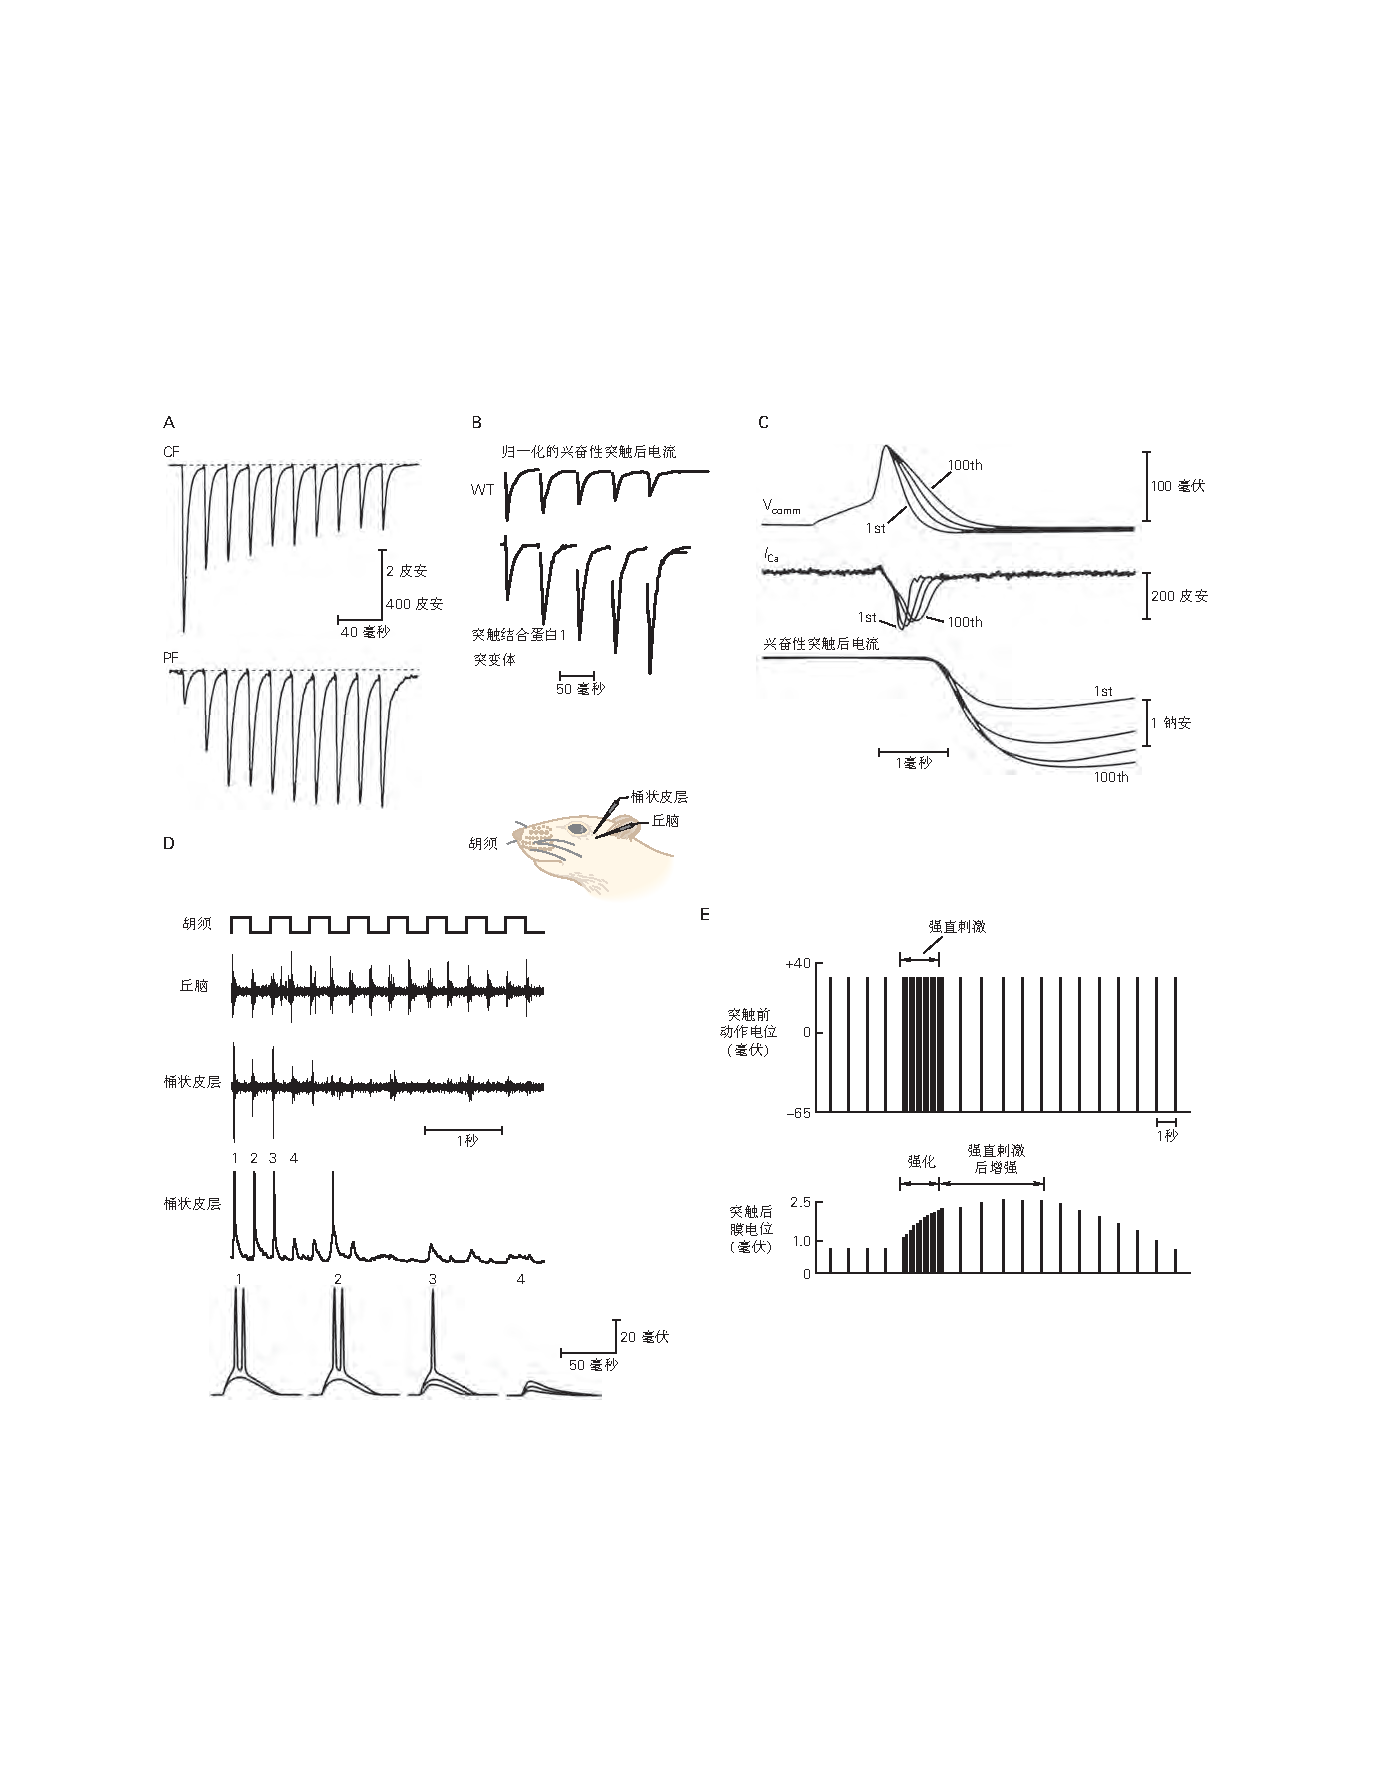
\includegraphics[width=0.9\linewidth]{chap15/fig_15_15}
	\caption{中枢神经系统短期可塑性的多样性。
		A. \textit{兴奋性突触后电流}是在电压钳下从小脑浦肯野神经元记录的,以响应对浦肯野细胞的\textit{攀缘纤维}或\textit{平行纤维}输入的重复刺激。
		在这 2 种情况下,\textit{兴奋性突触后电流}都被记录下来,而传入神经在 50 赫兹下被刺激 10 次。
		请注意,\textit{攀缘纤维}\textit{兴奋性突触后电流}抑制而\textit{平行纤维}\textit{兴奋性突触后电流}在重复刺激期间促进\cite{dittman2000interplay}。
		B. \textit{兴奋性突触后电流}在 20 赫兹的刺激过程中从培养的海马体神经元中记录下来。
		通过将每个响应除以每个单独序列中第一个\textit{兴奋性突触后电流}的峰值振幅,将\textit{兴奋性突触后电流}大小归一化。
		\textit{兴奋性突触后电流}抑制从\textit{野生型}小鼠培养的神经元,而\textit{兴奋性突触后电流}促进来自携带突变形式的\textit{突触结合蛋白}-1 的小鼠的神经元,该突触结合蛋白-1 降低其 \ce{Ca^2+} 结合亲和力(\textit{突触结合蛋白1}突变体,R233Q)\cite{fernandez2001synaptotagmin}。
		C. 在 2 秒长的 50 赫兹刺激序列中,齿状回颗粒神经元突触前末梢记录的动作电位逐渐变宽。
		这导致从颗粒神经元到它们的\textit{阿蒙角}3 突触后目标的突触传递增强。
		显示第 1、25、50 和 100 个动作电位。
		然后将这些动作电位波形用作命令波形($V_\text{comm}$,顶部)以电压钳制突触前神经末梢(“动作电位钳”),引发末梢(中间)和突触后\textit{阿蒙角}3 神经元中的\textit{兴奋性突触后电流}(底部)。
		随着动作电位波形持续时间的增加,$I_{Ca}$ 的持续时间增加,从而增加了\textit{兴奋性突触后电流}的振幅\cite{geiger2000dynamic}。
		D. 在对初级胡须进行一系列 4 赫兹机械刺激(顶部迹线)期间,同时对丘脑和桶状皮层的动作电位进行细胞外多单元记录(从顶部开始的第二条和第三条迹线)。
		皮层和丘脑响应在刺激过程中都会抑制,尽管皮层响应抑制得更快。
		晶须桶中皮层神经元对初级晶须 4 赫兹刺激的细胞内电压响应(底部两条迹线)。
		两条轨迹中的第一条显示了对一列序列中连续的晶须刺激的响应。
		时间刻度与顶部轨迹相同。
		底部轨迹显示了 3 个独立序列中对晶须刺激的前 4 个反应的扩展视图。
		请注意,对于序列中第二和第三刺激的脉冲反应,试验与试验之间存在差异,这可能是由于递质释放的概率性质\cite{chung2002short}。
		E. 高频刺激的短暂爆发导致递质释放的持续增强。
		此处实验记录的时间尺度已被压缩(每个突触前和突触后电位显示为一条线,表示其振幅)。
		当以每秒一个动作电位的相对较低的速率刺激突触前神经元时,会产生大约 1 毫伏的稳定\textit{兴奋性突触后电位}。
		然后以每秒 50 个动作电位的较高速率刺激突触前神经元几秒钟。
		在这种强直刺激期间,由于增强的递质释放,\textit{兴奋性突触后电位}的大小增加,这种现象称为增强。
		刺激几秒钟后,突触前神经元恢复到初始刺激速率(每秒一次)。
		然而,\textit{兴奋性突触后电位}会在几分钟内保持增强,在某些细胞中,甚至会持续几个小时。
		这种持续增加称为强直后增强。}
	\label{fig:15_15}
\end{figure}


这些技术提供了胞吐过程中活动区突触小泡的清晰图像。 
使用一种称为冷冻断裂电子显微镜的技术,\textit{里斯}和\textit{霍伊泽尔}注意到突触活动后突触前膜沿活动区立即发生变形,他们将其解释为突触小泡融合引起的细胞膜内陷。 
这些变形沿着 1 排或 2 排异常大的膜内颗粒分布,沿着突触前密度的 2 个边缘可见。
如图~\ref{fig:15_7}~所示,许多这些颗粒现在被认为是电压门控 \ce{Ca^2+} 通道。
颗粒密度(约 1,500 个/微米$ ^2 $)与被认为存在于活性区突触前细胞质膜中的 \ce{Ca^2+} 通道密度相似。
此外,粒子与释放位点的接近程度与 \ce{Ca^2+} 电流开始与递质释放之间的短时间间隔一致。


\begin{figure}[htbp]
	\centering
	\includegraphics[width=1.0\linewidth]{chap15/fig_15_7}
	\caption{突触小泡通过胞吐作用释放递质,并通过胞吞作用回收。
		左边的图像是神经肌肉接头处的冷冻断裂电子显微照片。
		冷冻断裂技术通过沿着脂质双层的疏水内部分裂膜来暴露膜内区域。
		如图~\ref{fig:15_4}A~所示,显示的视图是从突触间隙向上看的双层突触前膜的细胞质小叶。
		如图~\ref{fig:15_4}A~所示,右侧的传统薄层电子显微照片显示了突触前末梢、突触间隙和突触后肌膜的横截面视图\cite{heuser1981structural}。
		右侧的薄层图像显示了与活动区相邻的突触小泡。
		B. 突触小泡通过与细胞质膜融合(胞吐作用)释放递质。
		在这里,突触小泡在去极化刺激后 5 毫秒内通过快速冷冻组织而与细胞质膜融合。
		细胞质膜中的每个凹陷代表 1 个突触小泡的融合。
		在右侧的显微照片中,融合的囊泡被视为$\Omega$形结构。
		C. 胞吐作用后,突触小泡膜通过胞吞作用恢复。
		在囊泡与突触前膜融合后约 10 秒内,形成包被凹坑。
		再过 10 秒后,包被的凹坑开始通过内吞作用夹断,形成包被的囊泡。
		这些囊泡储存原始突触囊泡的膜蛋白以及从细胞外介质捕获的分子。
		囊泡在末梢被回收或被运输到细胞体,膜成分在细胞体中被降解或回收(见第~\ref{chap:chap7}~章)。}
	\label{fig:15_7}
\end{figure}



最后,\textit{霍伊泽尔}和\textit{里斯}发现这些变形是短暂的;
它们仅在囊泡排出时发生,并且在递质释放后不会持续存在。
如图~\ref{fig:15_7}B~所示,薄截面电子显微照片显示许多 $\Omega$ 形结构,在囊泡膜完全塌陷到细胞质膜之前,突触囊泡的外观刚刚与膜融合。
\textit{霍伊泽尔}和\textit{里斯}通过证明当他们改变 4-氨基吡啶的浓度以改变递质释放量时,$\Omega$形结构的数量与\textit{兴奋性突触后电位}的大小直接相关,从而证实了这一想法。
这些形态学研究提供了显著的证据,证明递质通过胞吐作用从突触小泡中释放出来。


在胞吐作用之后,回收添加到突触前末梢的多余膜。
如图~\ref{fig:15_7}C~所示,在刺激后 10 到 20 秒的突触前末梢图像中,\textit{霍伊泽尔}和\textit{里斯}观察到细胞质膜上的新结构(即涂层凹坑),这些凹坑由蛋白质网格蛋白形成,有助于通过内吞作用介导膜恢复。
几秒钟后,可以看到涂层凹坑从膜上夹断,并在细胞质中显示为涂层囊泡。
正如我们稍后将看到的,通过包被坑形成的内吞作用代表了囊泡膜修复的几种方法之一。



\subsection{电容测量提供了对胞吐和胞吞动力学的洞察力}

在具有大突触前末梢的某些神经元中,胞吐过程中细胞质膜表面积的增加可以在电测量中检测为膜电容的增加。
正如我们在第~\ref{chap:chap9}~章中看到的,膜的电容与其表面积成正比。
\textit{厄温$\cdot$内尔}发现可以使用电容测量来监测分泌细胞的胞吐作用。


在肾上腺嗜铬细胞(释放肾上腺素和去甲肾上腺素)和大鼠腹膜的肥大细胞(释放组胺和\textit{5-羟色氨})中,单个致密核心囊泡足够大,可以测量与单个囊泡融合相关的电容增加。
如图~\ref{fig:15_8}~所示,这些细胞中递质的释放伴随着电容的逐步增加,随后是逐步减少,这反映了多余膜的回收和再循环。


\begin{figure}[htbp]
	\centering
	\includegraphics[width=0.75\linewidth]{chap15/fig_15_8}
	\caption{电容的变化揭示了胞吐作用和胞吞作用的时间过程。
		A. 电子显微照片显示肥大细胞在胞吐作用之前(左)和之后(右)。
		肥大细胞是免疫系统的分泌细胞,其中包含充满递质组胺和\textit{5-羟色氨}的大致密核心囊泡。
		分泌囊泡的胞吐作用通常由与\textit{免疫球蛋白}复合的抗原结合触发。
		在实验条件下,细胞内记录电极中包含不可水解的\textit{三磷酸鸟苷}类似物可触发大量胞吐作用。
		B. 电容的逐步增加反映了单个分泌囊泡与肥大细胞膜的连续融合。
		由于囊泡膜面积的可变性,步骤增加是不相等的。
		胞吐作用后,通过融合添加的膜通过胞吞作用回收。
		单个囊泡的内吞作用导致膜电容逐步降低。
		以这种方式,细胞保持恒定的大小(单位为飞法拉,其中 1 fF = 0.1 平方微米膜面积)\cite{fernandez1984capacitance}。
		C. 视网膜中双极神经元的巨大突触前末梢超过 5 微米直径,允许膜电容和 \ce{Ca^2+} 电流的直接膜片钳记录。
		膜电位(毫伏)中的一个短暂的去极化电压钳步骤会引起持续的大 \ce{Ca^2+} 电流($I_{Ca}$)和细胞质 \ce{Ca^2+} 浓度 [Ca]$_i$ 的升高。
		这导致数千个小突触囊泡与细胞膜融合,导致总膜电容增加。
		由单个囊泡融合引起的电容增量太小而无法分辨。
		随着内部 \ce{Ca^2+} 浓度在复极化后回落到其静止水平,额外的膜面积被恢复并且电容返回到其基准值。
		由于内吞作用和 \ce{Ca^2+} 代谢相对缓慢,电容和 \ce{Ca^2+} 浓度的增加比短暂的去极化和 \ce{Ca^2+} 电流(注意不同的时间尺度)持续时间更长\cite{zenisek2004visualizing}。}
	\label{fig:15_8}
\end{figure}


在神经元中,由单个小突触囊泡融合引起的电容变化通常太小而无法分辨。
如图~\ref{fig:15_8}C~所示,在某些释放大量囊泡的有利突触制剂中(例如视网膜中双极神经元的巨大突触前末梢),膜去极化会触发末梢总电容的瞬时平滑上升和下降,这是由于从数百个单独的突触囊泡中胞吐和回收膜的结果。
这些结果提供了膜融合和修复率的直接测量。



\subsection{胞吐作用涉及临时融合孔的形成}

使用快速冷冻对肥大细胞的形态学研究表明:胞吐作用取决于跨越囊泡膜和细胞质膜的临时融合孔的形成。
在肥大细胞电容增加的电生理学研究中,在囊泡和细胞膜完全融合之前,在电生理学记录中检测到通道状融合孔。 
该融合孔以大约 200 皮西门子的单通道电导开始,类似于间隙连接通道,它也桥接 2 个膜。
如图~\ref{fig:15_9}A~所示,在胞吐过程中,孔迅速扩张,直径可能从 5 纳米到 50 纳米左右,电导急剧增加。


\begin{figure}[htbp]
	\centering
	\includegraphics[width=0.9\linewidth]{chap15/fig_15_9}
	\caption{融合孔的可逆打开和可逆关闭。
		A. 全细胞膜片钳用于记录与融合孔打开相关的膜电流。
		当囊泡与细胞质膜融合时,囊泡的电容($C_g$)最初通过融合孔($r_p$)的高电阻连接到细胞膜其余部分的电容($C_m$)。
		因为囊泡的膜电位(管腔侧负)通常比细胞的膜电位负得多,所以在融合过程中电荷从囊泡流向细胞膜。
		这种瞬态电流($I$)与膜电容($C_m$)的增加有关。
		根据 $\tau = C_g r_p = C_g / g_p$,可以根据瞬态电流的时间常数计算融合孔隙电导($g_p$)的大小。
		假设孔跨越 2 个脂质双层并充满电阻率等于细胞质电阻率的溶液,则可以根据孔隙电导计算孔径。
		右图显示孔的初始电导约为 200 皮西门子,类似于间隙连接通道的电导,对应于约 2 纳米的孔径。
		随着孔在 10 毫秒内扩张到大约 7 至 8 纳米(实心圆),孔径和电导率迅速增加\cite{monck1992exocytotic,spruce1990properties}。
		B. 递质释放通过安培法测量。
		细胞被全细胞贴片电极电压钳位,同时细胞外碳纤维被压在细胞表面。
		施加到碳电极尖端的大电压会氧化某些胺类递质(例如\textit{5-羟色氨}或去甲肾上腺素)。
		1 个分子的这种氧化会产生 1 个或多个自由电子,从而产生与递质释放量成正比的电流。
		可以通过连接到碳电极的放大器($A_2$)记录电流。
		膜电流和电容通过贴片电极放大器($A_1$)记录。
		肥大细胞分泌囊泡的\textit{5-羟色氨}释放(顶部迹线)和电容测量(底部迹线)的记录显示在右侧。
		记录表明,\textit{5-羟色氨}可能会在完全融合之前通过融合孔的可逆性打开和关闭而释放(左侧的迹线)。
		在这些短暂的开口期间,少量的递质通过孔逸出,导致在完全融合后释放大量递质之前的低电平信号(1 英尺)。
		在足部,随着融合孔的打开和关闭,细胞表面积(与膜电容成正比)经历可逆的阶梯状变化。
		有时,融合孔的可逆打开和关闭并没有完全融合(右侧的痕迹)。}
	\label{fig:15_9}
\end{figure}


融合孔不仅仅是导致递质胞吐的中间结构,因为递质可以在孔扩张和囊泡塌陷之前通过孔释放。
这首先通过安培法显示,这种方法使用细胞外碳纤维电极检测某些胺类神经递质(例如\textit{5-羟色氨}),基于递质和电极之间的电化学反应,产生与局部递质浓度成比例的电流。
5-羟色胺能细胞中动作电位的激发导致电极电流的大量瞬时增加,对应于单个致密核囊泡内容物的胞吐作用。
如图~\ref{fig:15_9}B~所示,在某些情况下,这些大的瞬态增加之前是较小、持续时间更长的电流信号,这些信号反映了递质通过融合孔的泄漏,融合孔在完全融合之前闪烁打开和关闭几次。


递质也可能仅通过短暂的融合孔释放,这些融合孔短暂地连接囊泡腔和细胞外空间,而囊泡膜不会完全塌陷到细胞质膜中。
神经内分泌细胞中大致密核囊泡胞吐作用的电容测量表明,融合孔可以快速且可逆地打开和关闭。
融合孔的可逆打开和关闭代表了一种非常快速的膜回收方法。
与全膜塌陷相反,快速突触处的小透明囊泡通过融合孔排出递质的情况尚不确定。



\subsection{突触小泡循环包括几个步骤}

当以高频发射时,典型的突触前神经元能够保持递质释放的高速率。
随着时间的推移,这可能导致大量囊泡的胞吐作用,超过突触前末梢形态学上明显的数量。
为了防止囊泡的供应在快速突触传递过程中迅速耗尽,使用过的囊泡会被迅速回收和回收。
因为神经末梢通常与细胞体有一段距离,所以通过细胞体中的合成来补充囊泡并运输到末梢会太慢而不适用于快速突触。


如图~\ref{fig:15_10}A~所示,突触小泡在一个简单的循环中被释放和重复使用。
囊泡充满神经递质并聚集在神经末梢。
然后它们停靠在活性区,在那里它们经历复杂的启动过程,使囊泡能够响应触发融合过程的 \ce{Ca^2+} 信号。
如图~\ref{fig:15_10}B~所示,存在许多机制用于在胞吐作用后恢复突触小泡膜,每个机制都有不同的时间过程。


\begin{figure}[htbp]
	\centering
	\includegraphics[width=0.85\linewidth]{chap15/fig_15_10}
	\caption{突触小泡周期。
		A. 突触小泡通过主动运输充满神经递质(第 1 步)并加入可能代表储备池的小泡簇(第 2 步)。
		填充的囊泡停靠在活性区(第 3 步),在那里它们经历\textit{三磷酸腺苷}依赖性启动反应(第 4 步),使它们能够进行 \ce{Ca^2+} 触发的融合(第 5 步)。
		释放内容物后,突触小泡通过几种通路之一循环(参见 B 部分)。
		在一种常见的通路中,囊泡膜通过网格蛋白介导的内吞作用(步骤 6)回收并直接回收(步骤 7)或通过核内体(步骤 8)回收。
		B. 递质放电后囊泡的恢复被认为是通过 3 种机制发生的,每种机制都有不同的动力学。
		1. 可逆融合孔是再利用囊泡的最快速机制。
		囊泡膜不与细胞质膜完全融合,递质通过融合孔释放。
		囊泡回收只需要关闭融合孔,因此可以在数十到数百毫秒内迅速发生。
		该通路可能在较低至正常的释放速率下占主导地位。
		用过的囊泡可能会留在膜上(亲吻和停留)或从膜重新定位到囊泡储备池(亲吻和奔跑)。
		2. 在经典通路中,多余的膜通过网格蛋白包被的小坑通过内吞作用回收。
		除了活动区外,这些凹坑遍布整个轴突末梢。
		该通路在正常到高释放率下可能很重要。
		3. 在大量回收通路中,多余的膜通过未包被的凹坑出芽重新进入末梢。
		这些未涂层的池主要在活动区形成。
		该通路可能仅在高释放率之后使用,而不是在突触的正常功能期间使用\cite{schweizer1995vesicle}。}
	\label{fig:15_10}
\end{figure}


第一个也是最快速的机制涉及融合孔的可逆打开和关闭,而囊泡膜与细胞质膜没有完全融合。
在亲吻并停留通路中,融合孔关闭后囊泡保留在活性区,为第二次释放事件做好准备。
在\textit{亲完就跑}通路中,囊泡在融合孔关闭后离开活性区,但能够快速再释放。
这些通路被认为在低频刺激期间优先使用。


\textit{约根森}及其同事描述了超快网格蛋白非依赖性内吞作用的第二条通路,该通路比经典的网格蛋白介导通路快 200 倍。
在胞吐作用后仅 50 毫秒开始,超快胞吞作用就发生在活性区外。


较高频率的刺激会募集第三条较慢的回收通路,该通路使用网格蛋白在与细胞质膜融合后回收囊泡膜。
网格蛋白在内吞作用期间形成围绕膜的晶格状结构,从而在\textit{霍伊泽尔}和\textit{里斯}观察到的涂层凹坑周围出现涂层。
在此通路中,回收的囊泡膜必须通过内体隔室再循环,然后才能重复使用囊泡。
如图~\ref{fig:15_7}~所示,网格蛋白介导的循环需要最多 1 分钟才能完成,并且似乎也从活性区转移到活性区周围的膜上。
第四种机制在长时间的高频刺激后起作用。
在这些条件下,可以看到大量膜内陷进入突触前末梢,这被认为反映了膜通过称为批量回收的过程进行再循环。



\section{突触囊泡的胞吐仰仗高度保守的蛋白结构}

突触小泡的许多关键蛋白及其在细胞质膜中的相互作用伙伴已被分离和纯化。
如图~\ref{fig:15_11}~所示,分离的突触小泡的蛋白质组学分析提供了它们包含的多种蛋白质的普查。
2 种最丰富的蛋白质,\textit{突触泡蛋白}和\textit{突触结合蛋白}-1,参与囊泡融合,稍后讨论。
另一类重要的囊泡蛋白是神经递质转运蛋白(第~\ref{chap:chap16}~章)。
这些跨膜蛋白(以谷氨酸转运蛋白 v-GluT 为例)利用存储在电化学梯度中的能量使质子从细胞质中逆浓度梯度泵送递质分子进入囊泡。
质子动力由囊泡 \ce{H+} 泵 V-ATPase 产生,它将质子从细胞质泵入囊泡腔,导致囊泡酸碱值约为 5.0 的酸性。


\begin{figure}[htbp]
	\centering
	\includegraphics[width=0.84\linewidth]{chap15/fig_15_11}
	\caption{胞吐作用的分子成分。
		A. 谷氨酸能突触小泡的蛋白质成分描述(及其近似拷贝数)。
		蛋白质嵌入突触小泡中,按比例绘制。
		成分包括囊泡\textit{三磷酸腺苷}酶(每个囊泡 1-2 个)、\textit{囊泡谷氨酸转运蛋白}(每个囊泡约 10 个)、\textit{小突触囊泡蛋白}(每个囊泡约 70 个)、\textit{突触结合蛋白}(每个囊泡约 15 个)和 小 GTPases Rab3 和/或 Rab27。
		估计值是作为许多囊泡的平均值获得的\cite{takamori2006molecular}。
		B. 介导 \ce{Ca^2+} 触发的囊泡与突触前细胞膜融合的分子机制。
		这种对停靠突触小泡和突触前活动区的一部分的描述说明了神经递质释放机制的几个关键功能蛋白的相互作用。
		右图:虚线框显示核心融合机制,由\textit{可溶性N-乙基马来酰亚胺敏感因子附着受体}蛋白\textit{突触泡蛋白}/\textit{突触小泡缔合性膜蛋白}、\textit{突触融合蛋白}-1 和\textit{可溶性N-乙基马来酰亚胺敏感因子附着受体}-25 以及\textit{哺乳动物非协调蛋白}18-1 组成。
		\ce{Ca^2+} 传感器\textit{突触结合蛋白}-1 与 complexin(显示为与\textit{可溶性N-乙基马来酰亚胺敏感因子附着受体}复合体结合)协同作用。
		左图:活性区蛋白复合物还包含\textit{Rab相互作用分子}、\textit{哺乳动物非协调蛋白13}和\textit{Rab相互作用分子结合蛋白}以及突触前细胞质膜中的 \ce{Ca^2+} 通道。
		\textit{Rab相互作用分子}在这个复合物中起着核心作用,通过结合特定的靶蛋白来协调活性区的多种功能:
		(1)囊泡 Rab 蛋白(Rab3 和 Rab27)介导囊泡对接;
		(2)\textit{哺乳动物非协调蛋白13}激活囊泡启动;
		(3)\ce{Ca^2+} 通道,直接和间接通过\textit{Rab相互作用分子结合蛋白},将 \ce{Ca^2+} 通道束缚在对接囊泡 100 纳米以内。
		活性区蛋白复合物将关键元素放入附近,使囊泡能够快速停靠、引发和融合,以响应动作电位,触发的 \ce{Ca^2+}进入停靠囊泡附近\cite{sudhof2013neurotransmitter}。}
	\label{fig:15_11}
\end{figure}


其他突触小泡蛋白将小泡引导至它们的释放位点,通过胞吐作用参与递质的释放,并介导小泡膜的再循环。
这 3 个步骤中涉及的蛋白质机制在从蠕虫到人类的整个进化过程中都得到了保护,并构成了神经递质调节释放的基础。
我们依次考虑这些步骤中的每一个。



\subsection{突触蛋白对囊泡的抑制和动员很重要}

活性区外的囊泡代表递质储备池。
\textit{保罗$\cdot$格林加德}发现了一个蛋白质家族(即突触蛋白),它们被认为是囊泡储备池的重要调节剂。
突触蛋白是与突触小泡的细胞质表面结合的外周膜蛋白。
突触蛋白包含一个保守的中央\textit{三磷酸腺苷酶}结构域,占其结构的大部分,但其功能仍然未知。
此外,\textit{突触素}-1 结合肌动蛋白。


突触蛋白是蛋白激酶 A 和 \ce{Ca^2+}/钙调蛋白依赖性蛋白激酶 II 的底物。
当神经末梢去极化并且 \ce{Ca^2+} 进入时,突触蛋白被激酶磷酸化,从而从囊泡中释放出来。
引人注目的是,刺激突触蛋白磷酸化、突触蛋白基因缺失或细胞内注射突触蛋白抗体会导致神经末梢突触小泡数量减少,并导致神经末梢在重复刺激期间维持高递质释放率的能力下降。



\subsection{\textit{可溶性N-乙基马来酰亚胺敏感因子附着受体}蛋白催化囊泡与细胞质膜融合}

因为膜双层是稳定的结构,突触小泡和细胞质膜的融合必须克服大的不利活化能。
如图~\ref{fig:15_12}~所示,这是通过现在称为\textit{可溶性N-乙基马来酰亚胺敏感因子附着受体}的融合蛋白家族实现的。


\begin{figure}[htbp]
	\centering
	\includegraphics[width=0.95\linewidth]{chap15/fig_15_12}
	\caption{\textit{可溶性N-乙基马来酰亚胺敏感因子附着受体}复合体的形成和解离驱动突触小泡和细胞质膜的融合\cite{rizo2002snares}。
		 A. \textit{可溶性N-乙基马来酰亚胺敏感因子附着受体}循环。
		 1. \textit{突触泡蛋白}与 2 种细胞质膜蛋白相互作用,即跨膜蛋白突触融合蛋白和外周膜蛋白 \textit{可溶性N-乙基马来酰亚胺敏感因子附着受体}-25。
		 2. 这 3 种蛋白质形成紧密的复合物,使囊泡和突触前膜紧密并列。
		 \textit{哺乳动物非协调蛋白18}与\textit{可溶性N-乙基马来酰亚胺敏感因子附着受体}复合体结合。
		 3. \ce{Ca^2+}流入引发囊泡和细胞质膜的快速融合;
		 \textit{可溶性N-乙基马来酰亚胺敏感因子附着受体}复合体现在位于细胞质膜中。
		 4. 2 种蛋白质\textit{N-乙基顺丁烯二酰亚胺敏感性的融合蛋白}和 \textit{可溶性N-乙基马来酰亚胺敏感因子附着受体}(与 \textit{可溶性N-乙基马来酰亚胺敏感因子附着受体}-25 无关)与\textit{可溶性N-乙基马来酰亚胺敏感因子附着受体}复合体结合并导致它在\textit{三磷酸腺苷}依赖性反应中解离。
		 B. \textit{可溶性N-乙基马来酰亚胺敏感因子附着受体}复合体由一束 4 个 $\alpha$-螺旋组成,一个来自\textit{突触泡蛋白}和\textit{突触融合蛋白}, 2 个来自 \textit{可溶性N-乙基马来酰亚胺敏感因子附着受体}-25。
		 这里显示的结构是融合前的停靠囊泡(跨膜结构域的实际结构尚未确定,但出于说明目的,此处将结构域与囊泡和细胞质膜一起绘制)。}
	\label{fig:15_12}
\end{figure}


从酵母到人类,\textit{可溶性N-乙基马来酰亚胺敏感因子附着受体}普遍参与膜融合。
它们介导蛋白质从内质网到高尔基体再到细胞质膜的运动过程中的组成型膜运输,以及对调节胞吐作用很重要的突触小泡运输。
\textit{可溶性N-乙基马来酰亚胺敏感因子附着受体}具有一个保守的蛋白质序列,即\textit{可溶性N-乙基马来酰亚胺敏感因子附着受体}基序,其长度为 60 个残基。
它们有 2 种形式。
囊泡\textit{靶膜可溶性N-乙基马来酰亚胺敏感因子附着受体}或 v-\textit{靶膜可溶性N-乙基马来酰亚胺敏感因子附着受体}(也称为 R-\textit{靶膜可溶性N-乙基马来酰亚胺敏感因子附着受体},因为它们含有重要的中央精氨酸残基)位于囊泡膜中。
靶膜\textit{靶膜可溶性N-乙基马来酰亚胺敏感因子附着受体}或\textit{靶膜可溶性N-乙基马来酰亚胺敏感因子附着受体}(也称为Q-\textit{靶膜可溶性N-乙基马来酰亚胺敏感因子附着受体},因为它们含有重要的谷氨酰胺残基)存在于靶膜中(例如细胞质膜)。


每个突触小泡都包含一个称为\textit{突触泡蛋白}(也称为小泡相关膜蛋白或\textit{突触小泡缔合性膜蛋白})的 v-\textit{靶膜可溶性N-乙基马来酰亚胺敏感因子附着受体}。
相比之下,突触前活动区包含 2 种类型的\textit{靶膜可溶性N-乙基马来酰亚胺敏感因子附着受体}蛋白,\textit{突触融合蛋白}和 \textit{可溶性N-乙基马来酰亚胺敏感因子附着受体}-25(Synaptobrevin 和\textit{突触融合蛋白}有一个\textit{可溶性N-乙基马来酰亚胺敏感因子附着受体}基序;\textit{可溶性N-乙基马来酰亚胺敏感因子附着受体}-25 有 2 个)。
\textit{突触泡蛋白}、\textit{突触融合蛋白}和 \textit{可溶性N-乙基马来酰亚胺敏感因子附着受体}-25 都参与突触小泡与细胞质膜融合的第一个线索来自以下发现:
所有 3 种蛋白质都是肉毒杆菌毒素和破伤风毒素的底物,细菌蛋白酶是递质释放的有效抑制剂。
\textit{詹姆斯$\cdot$罗斯曼}随后提供了重要的见解,即这 3 种蛋白质在紧密的生化复合物中相互作用。
如图~\ref{fig:15_12}B~所示,在溶液中使用纯化的 v-SNARE 和\textit{靶膜可溶性N-乙基马来酰亚胺敏感因子附着受体}的实验中,4 个\textit{可溶性N-乙基马来酰亚胺敏感因子附着受体}基序彼此紧密结合形成$\alpha$-螺旋卷曲螺旋复合体。


\textit{可溶性N-乙基马来酰亚胺敏感因子附着受体}复合体的形成如何驱动突触小泡融合?
如图~\ref{fig:15_12}B~所示,在胞吐过程中,突触小泡上\textit{突触泡蛋白}的\textit{可溶性N-乙基马来酰亚胺敏感因子附着受体}基序与细胞质膜上的 \textit{可溶性N-乙基马来酰亚胺敏感因子附着受体}-25 和\textit{突触融合蛋白}的\textit{可溶性N-乙基马来酰亚胺敏感因子附着受体}基序形成紧密的复合体。
\textit{可溶性N-乙基马来酰亚胺敏感因子附着受体}复合物的晶体结构表明该复合物将膜聚集在一起。
\textit{突触泡蛋白}、\textit{突触融合蛋白}和 \textit{可溶性N-乙基马来酰亚胺敏感因子附着受体}-25 的三元复合物非常稳定。
如图~\ref{fig:15_12}~所示,其组装中释放的能量被认为会吸引囊泡和细胞质膜的带负电荷的磷脂紧密并置,迫使它们进入融合前的中间状态。
这种不稳定状态可能会开始形成融合孔,并产生在电生理测量中观察到的融合孔的快速打开和关闭(闪烁)。


然而,\textit{可溶性N-乙基马来酰亚胺敏感因子附着受体}并不能完全解释突触小泡和细胞质膜的融合。
脂质囊泡中纯化蛋白的重组实验表明突触小蛋白、\textit{突触融合蛋白}和 \textit{可溶性N-乙基马来酰亚胺敏感因子附着受体}-25 可以催化融合,但体外反应显示 \ce{Ca^2+} 几乎没有调节作用,并且反应比真实突触中的囊泡融合慢得多,效率也低得多。
突触小泡胞吐所需的一种重要的额外蛋白质是\textit{哺乳动物非协调蛋白18}(哺乳动物 unc18 同系物)。
\textit{哺乳动物非协调蛋白18} 的同系物,称为\textit{血清粘蛋白}(sec1/\textit{哺乳动物非协调蛋白18} 样蛋白),对于所有\textit{可溶性N-乙基马来酰亚胺敏感因子附着受体}介导的细胞内融合反应都是必不可少的。
\textit{哺乳动物非协调蛋白18}在\textit{可溶性N-乙基马来酰亚胺敏感因子附着受体}复合体组装之前与突触融合蛋白结合。
删除\textit{哺乳动物非协调蛋白18}会阻止神经元中的所有突触融合。
因此,核心融合机制由\textit{可溶性N-乙基马来酰亚胺敏感因子附着受体}和\textit{血清粘蛋白}组成,这些蛋白由特定融合响应特异的各种辅助因子调节。
最后,突触\textit{可溶性N-乙基马来酰亚胺敏感因子附着受体}复合物还与一种称为复合蛋白的小可溶性蛋白相互作用,后者抑制递质的自发释放,但增强~\ce{Ca^2+} 依赖性诱发释放。


融合后,必须拆解\textit{可溶性N-乙基马来酰亚胺敏感因子附着受体}复合体才能进行有效的囊泡回收。
\textit{罗斯曼}发现一种称为\textit{N-乙基顺丁烯二酰亚胺敏感性的融合蛋白}的细胞质\textit{三磷酸腺苷}酶通过一种称为 \textit{可溶性N-乙基马来酰亚胺敏感因子附着受体}(可溶性 NSF 附着蛋白,与\textit{可溶性N-乙基马来酰亚胺敏感因子附着受体}蛋白 \textit{可溶性N-乙基马来酰亚胺敏感因子附着受体}-25 无关)的衔接蛋白与\textit{可溶性N-乙基马来酰亚胺敏感因子附着受体}复合物结合。
如图~\ref{fig:15_12}A~所示,\textit{N-乙基顺丁烯二酰亚胺敏感性的融合蛋白}和\textit{可溶性N-乙基马来酰亚胺敏感因子附着受体}使用\textit{三磷酸腺苷}水解的能量来解离\textit{可溶性N-乙基马来酰亚胺敏感因子附着受体}复合物,从而再生游离\textit{可溶性N-乙基马来酰亚胺敏感因子附着受体}。
\textit{可溶性N-乙基马来酰亚胺敏感因子附着受体}和\textit{N-乙基顺丁烯二酰亚胺敏感性的融合蛋白}还参与树突棘中突触后\textit{$\alpha$-氨基-3-羟基-5-甲基-4-异恶唑丙酸}型谷氨酸受体的循环。



\subsection{\ce{Ca^2+}与突触结合蛋白的结合触发递质释放}

因为突触小泡与细胞质膜的融合必须在几分之一毫秒内发生,所以人们认为大多数负责融合的蛋白质在 \ce{Ca^2+} 流入之前组装。
根据这一观点,一旦 \ce{Ca^2+} 进入突触前末梢,它就会与囊泡上的 \ce{Ca^2+} 传感器结合,立即触发膜融合。


一个密切相关的蛋白质家族的成员(即突触结合蛋白),已被确定为触发突触小泡融合的主要 \ce{Ca^2+} 传感器。
如图~\ref{fig:15_13}A、B~所示,突触结合蛋白是具有单个 N 末梢跨膜区的膜蛋白,可将它们固定在突触小泡上。
每个突触结合蛋白的细胞质区域主要由 2 个结构域组成(即 C2 结构域),这是与蛋白激酶 C 的 \ce{Ca^2+} 和磷脂结合 C2 结构域同源的常见蛋白质基序。
发现 C2 结构域不仅结合 \ce{Ca^2+},而且结合 磷脂也与其在 \ce{Ca^2+} 依赖性胞吐作用中的重要性一致。
\textit{突触结合蛋白}-1、\textit{突触结合蛋白}-2 和 \textit{突触结合蛋白}-9 已被确定为用于快速同步囊泡融合的 \ce{Ca^2+} 传感器。
每个都表现出不同的 \ce{Ca^2+} 结合亲和力和动力学,根据表达的特定突触结合蛋白亚型赋予不同的突触不同的释放特性。
相比之下,\textit{突触结合蛋白}-7 介导一种较慢形式的 \ce{Ca^2+} 触发的胞吐作用,这种胞吐作用对于重复触发动作电位的长时间活动期间的突触传递很重要。
所有这些突触结合蛋白还在其他形式的胞吐作用中充当 \ce{Ca^2+} 传感器,例如内分泌细胞中的胞吐作用和 \textit{$\alpha$-氨基-3-羟基-5-甲基-4-异恶唑丙酸}型谷氨酸受体在\textit{N-甲基-D-天冬氨酸}受体依赖性\textit{长时程增强}期间从细胞内囊泡池插入突触后细胞膜。


对突触结合蛋白-1 被删除或通过基因工程改变其 \ce{Ca^2+} 亲和力的突变小鼠的研究提供了重要证据,证明突触结合蛋白是生理 \ce{Ca^2+} 传感器。
当突触结合蛋白对 \ce{Ca^2+} 的亲和力降低 2 倍时,递质释放所需的 \ce{Ca^2+} 会发生相同数量的变化。
当小鼠、果蝇或蠕虫中的\textit{突触结合蛋白}-1 被删除时,动作电位不再能够触发快速同步释放。
然而,如图~\ref{fig:15_13}A~所示,\ce{Ca^2+} 仍然能够刺激一种较慢形式的递质释放(称为异步释放),由\textit{突触结合蛋白}-7 介导。
因此,几乎所有 \ce{Ca^2+} 触发的神经递质释放都依赖于突触结合蛋白。


\begin{figure}[htbp]
	\centering
	\includegraphics[width=0.95\linewidth]{chap15/fig_15_13}
	\caption{突触结合蛋白通过形成有利于囊泡融合的蛋白质复合物来介导 \ce{Ca^2+} 依赖性递质释放。
		A. 缺乏\textit{突触结合蛋白}-1 的突变小鼠不存在快速 \ce{Ca^2+} 触发的递质释放。
		记录显示兴奋性突触后电流通过刺激来自野生型小鼠和突变小鼠的培养的海马体神经元在体外诱发,其中 \textit{突触结合蛋白}-1 已通过同源重组(1)被删除。
		来自野生型小鼠的神经元显示出由突触前动作电位诱发的大而快速的兴奋性突触后电流,反映了突触传递受大量突触小泡快速同步释放递质支配的事实。
		在底部轨迹(2)中,突触电流以高度扩展的比例显示,可以看到同步释放的快速阶段之后是一个小的、延长的递质异步释放阶段。
		在这个缓慢的阶段,个体量子响应的频率会持续增加。
		在突变小鼠的神经元中,突触前动作电位仅触发缓慢的异步释放阶段;
		快速同步阶段已被废除\cite{geppert1994synaptotagmin}。
		B. X 射线晶体结构突触结合蛋白。
		B1. 带状图显示 C2A 结构域结合 3 个 \ce{Ca^2+},C2B 结构域结合 2 个 \ce{Ca^2+}。
		蓝色箭头表示 $\beta$ 链。
		在 C2B 结构域的 C 末梢有 2 个短的 $\alpha$-螺旋(橙色)。
		突触结合蛋白其他区域的结构尚未确定,在此绘制以供说明之用。
		膜和结构按比例绘制\cite{fernandez2001three}。
		B2. 与\textit{可溶性N-乙基马来酰亚胺敏感因子附着受体}复合物(\textit{突触泡蛋白}、\textit{突触融合蛋白}和\textit{可溶性N-乙基马来酰亚胺敏感因子附着受体}-25)和 complexin 结合的突触结合蛋白(浅蓝色)的 X 射线晶体结构。
		未显示突触结合蛋白的跨膜结构域\cite{zhou2017primed}。
		C. 突触结合蛋白-复合蛋白-\textit{可溶性N-乙基马来酰亚胺敏感因子附着受体}复合物的拉链介导囊泡融合。
		顶部,在没有 \ce{Ca^2+} 的情况下,\textit{可溶性N-乙基马来酰亚胺敏感因子附着受体}复合体和复合体的 $\alpha$-螺旋与结合的突触结合蛋白仅部分拉开。
		中间,\ce{Ca^2+} 与突触结合蛋白的 C2A 和 C2B 结构域的结合使它们能够与细胞质膜相互作用,施加力使囊泡和细胞质膜靠得更近。
		底部,突触结合蛋白介导的接近和复合物-\textit{可溶性N-乙基马来酰亚胺敏感因子附着受体}-突触结合蛋白复合物的最终拉链触发膜融合\cite{zhou2017primed}。}
	\label{fig:15_13}
\end{figure}


\ce{Ca^2+} 与突触结合蛋白的结合如何触发囊泡融合?
如图~\ref{fig:15_13}B~所示,2 个 C2 结构域结合总共 5 个 \ce{Ca^2+},与触发递质量子释放所需的最少 \ce{Ca^2+} 数量相同。
然而,由于多个突触结合蛋白可能参与触发释放,超过 5 个结合的 \ce{Ca^2+} 可能分布在单个囊泡上的多个突触结合蛋白分子中。


\ce{Ca^2+} 与突触结合蛋白的结合被认为充当开关,促进 C2 结构域与磷脂的相互作用。
突触结合蛋白的 C2 结构域也与\textit{可溶性N-乙基马来酰亚胺敏感因子附着受体}蛋白和复合蛋白相互作用。
突触结合蛋白的晶体结构揭示了与相关\textit{可溶性N-乙基马来酰亚胺敏感因子附着受体}复合体的保守主界面。
此外,第 2 个突触结合蛋白分子与相同的\textit{可溶性N-乙基马来酰亚胺敏感因子附着受体}复合物和络合物形成三方相互作用。
\textit{布伦杰}及其同事发现:主要的\textit{可溶性N-乙基马来酰亚胺敏感因子附着受体}复合物/突触结合蛋白界面和三方\textit{可溶性N-乙基马来酰亚胺敏感因子附着受体}复合物/突触结合蛋白/复合蛋白界面对于快速 \ce{Ca^2+} 触发的融合都是必不可少的。
这些发现导致了以下假设:
(1)在静止时,启动囊泡的突触结合蛋白存在于具有部分预拉链的\textit{可溶性N-乙基马来酰亚胺敏感因子附着受体}蛋白和络合物的复合物中;
(2)在动作电位触发的 \ce{Ca^2+} 流入后,\ce{Ca^2+} 与突触结合蛋白结合。
这触发了突触结合蛋白和细胞质膜之间的相互作用,导致复合物整体旋转,从而诱导复合物部分从\textit{可溶性N-乙基马来酰亚胺敏感因子附着受体}复合物上解离;
(3)如图~\ref{fig:15_13}C~所示,这种旋转导致细胞质膜凹陷,其面向细胞质的脂质重新排列,并最终导致细胞质膜和囊泡膜融合。
通过这种方式,可以利用突触结合蛋白、\ce{Ca^2+} 和膜的有利相互作用的能量来解除络合物介导的融合锁定并促进囊泡膜与细胞质膜的能量不利合并。



\subsection{融合机制嵌入在活性区的保守蛋白质支架中}

正如我们所见,快速突触传递的一个决定性特征是神经递质在活动区通过胞吐作用释放。
其他类型的胞吐作用(例如发生在肾上腺髓质中的胞吐作用)不需要细胞质膜的专门区域。
活性区被认为可以协调和调节突触小泡的对接和启动,以实现释放的速度和严格调节。
这是通过一组保守的蛋白质来实现的,这些蛋白质在活性区形成一个大的大分子结构。


\textit{杰克$\cdot$马克汉}使用一种称为电子显微断层扫描的强大超微结构技术,获得了青蛙神经肌肉接头处活动区的精美细节视图。
如图~\ref{fig:15_14}~所示,该技术展示了突触小泡如何通过一系列独特的结构实体(称为肋骨和横梁)束缚在膜上,这些结构实体附着在小泡上的特定位置和突触前膜中的颗粒(钉子)上,这些颗粒可能对应于电压门控 \ce{Ca^2+} 通道。


\begin{figure}[htbp]
	\centering
	\includegraphics[width=1.0\linewidth]{chap15/fig_15_14}
	\caption{活动区的突触小泡。
		图像是从电子显微镜断层扫描获得的\cite{harlow2001architecture}。
		A. 囊泡与活性区的丝状蛋白相连。
		解决了 3 种不同的丝状结构:钉子、肋骨和横梁。
		从囊泡突出的肋骨连接到长的水平横梁上,这些梁通过垂直销钉固定在膜上。
		B. 叠加在活性区膜内颗粒冻结断裂视图上的肋骨和横梁显示了肋骨如何与颗粒对齐,其中一些被认为是电压门控\ce{Ca^2+}通道。
		C. 活动区结构的模型显示了突触小泡、钉子、肋骨和横梁之间的关系。}
	\label{fig:15_14}
\end{figure}


了解各种突触小泡和活性区蛋白在胞吐过程中如何协调的一个关键目标是将已识别的各种蛋白质与该电子显微结构的元素相匹配。
已经鉴定出几种细胞质蛋白,它们被认为是活性区结构基质的组分。
这些包括 3 个大的细胞质多结构域蛋白,\textit{哺乳动物非协调蛋白13}(与前面讨论的\textit{哺乳动物非协调蛋白18}蛋白无关)、\textit{Rab相互作用分子}和\textit{Rab相互作用分子结合蛋白},它们彼此形成紧密的复合体,可能构成肋骨和横梁的一部分 。
突触小泡与\textit{Rab相互作用分子}和\textit{哺乳动物非协调蛋白13}的结合对于启动小泡进行胞吐作用至关重要。
\textit{环磷酸腺苷}依赖性蛋白激酶对\textit{Rab相互作用分子}的磷酸化与增强与可能有助于学习和记忆的某些形式的长期突触可塑性相关的递质释放有关。
正如我们稍后将看到的,第二信使对\textit{哺乳动物非协调蛋白13}的调节涉及突触可塑性的短期形式。


\textit{Rab相互作用分子}结合突触小泡蛋白 Rab3 和 Rab27,它们是低分子量鸟苷三磷酸酶(GTPases)家族的成员。
如图~\ref{fig:15_11}B~所示,Rab3 和 Rab27 蛋白作为\textit{三磷酸鸟苷}结合的 Rab3 复合物与突触小泡瞬时结合。
\textit{Rab相互作用分子}与 Rab3 或 Rab27 的结合被认为在\textit{可溶性N-乙基马来酰亚胺敏感因子附着受体}复合体组装之前的囊泡周期中将突触囊泡束缚在活性区。
此外,\textit{Rab相互作用分子}和\textit{Rab相互作用分子结合蛋白}共同调节 \ce{Ca^2+} 通道向活性区的募集,从而使 \ce{Ca^2+} 流入与囊泡释放紧密耦合。
这种通用机制在进化过程中得以保存,并且存在于无脊椎动物中,尽管有所修改。



\section{递质释放的调控是突触可塑性的基础}

化学突触的有效性可以被显著和快速地调节(在几秒钟内调节几倍),而且这种变化可以维持几秒钟、几小时、甚至几天或更长时间,这种特性称为突触可塑性。


突触强度可以通过改变神经递质的释放在突触前进行修改,也可以在突触后通过调节对递质的反应(如第~\ref{chap:chap13}~章所述)进行修改,或两者兼而有之。
突触前和突触后机制的长期变化对于发育过程中突触连接的完善(第~\ref{chap:chap49}~章)以及学习和记忆过程中的信息存储(第~\ref{chap:chap53}~和~\ref{chap:chap54}~章)至关重要。
在这里,我们关注如何通过调制释放的递质数量来改变突触强度。
原则上,递质释放的变化可以通过 2 种不同的机制介导:
\ce{Ca^2+} 流入的变化或响应给定 \ce{Ca^2+} 浓度而释放的递质数量的变化。
正如我们稍后将看到的,2 种类型的机制都有助于不同形式的可塑性。


突触强度通常会因突触前神经元的活动模式而改变。
如图~\ref{fig:15_15}A~所示,动作电位序列在一些突触处产生连续较大的突触后电流,在其他突触处产生连续较小的电流。
对重复刺激的突触后反应大小的减小称为突触抑制(图~\ref{fig:15_15}A,上图);
相反,通过重复刺激增强传递,称为突触促进或增强(图~\ref{fig:15_15}A,下图,\ref{fig:15_15}E)。
如图~\ref{fig:15_15}A~所示,各种突触表现出这些不同形式的短期突触可塑性(有时重叠,有时以一种为主),导致个别突触类型的短期动力学特征模式。


突触是促进还是抑制通常取决于响应序列的第一动作电位的释放概率。
具有初始高释放概率的突触通常会受到抑制,因为高释放率会暂时耗尽活动区的对接囊泡。
初始释放概率较低的突触会经历突触促进,部分原因是细胞内 \ce{Ca^2+} 在训练过程中的积累增加了释放的概率(见下文)。
从基因突变的影响可以看出释放概率在控制可塑性符号中的重要性。
由细胞培养物中的海马体神经元形成的突触最初具有较高的释放概率,因此通常会响应 20 赫兹的刺激而抑制。
然而,如图~\ref{fig:15_15}B~所示,将\textit{突触结合蛋白}-1 的 \ce{Ca^2+} 结合亲和力降低大约 2 倍的突变,从而降低了释放的初始概率,将抑制突触转化为促进突触。


影响突触前末梢游离 \ce{Ca^2+} 浓度的机制也会影响释放的递质数量。
例如,高频放电期间某些电压门控 \ce{K+} 通道失活的累积导致动作电位持续时间逐渐增加。
如图~\ref{fig:15_15}C~所示,动作电位的延长会增加电压门控 \ce{Ca^2+} 通道保持开放的时间,从而导致 \ce{Ca^2+} 的进入增强和随后递质释放的增加,从而导致更大的突触后电位。


大多数关于短期突触动力学的功能影响的研究都是在体外进行的或基于计算结果。
然而,最近的体内实验开始揭示短期可塑性的行为重要性。
例如,来自丘脑皮层突触的啮齿类动物的体内记录表明:突触抑制可能有助于反复刺激胡须期间的感觉适应。
如图~\ref{fig:15_15}D~所示,这种感觉适应的时间过程与皮层脉冲信号对晶须刺激的减弱和丘脑皮层突触中\textit{兴奋性突触后电位}的突触抑制并行。


突触前神经元的高频刺激在某些细胞中每秒可产生高达 5 百至 1 千个动作电位,称为强直刺激。
如此强烈的刺激会引起突触强度的显著变化。
强直刺激期间\textit{兴奋性突触后电位}大小的增加称为增强;
如图~\ref{fig:15_15}E~所示,强直刺激后持续增加称为强直后增强。
与持续几毫秒到几秒的突触促进相反,强直后增强通常持续几分钟,但它可以在某些突触处持续一个小时或更长时间。


突触利用包含\textit{哺乳动物非协调蛋白13}和\textit{Rab相互作用分子}(前面讨论的 2 种活性区蛋白)的复合物来抵消高频刺激期间的囊泡耗竭。
\textit{强直刺激}期间突触前 \ce{Ca^2+} 的升高会激活磷脂酶 C,从而产生\textit{肌醇1,4,5-三磷酸}和甘油二酯。
二酰甘油直接与\textit{哺乳动物非协调蛋白13}上称为 C1 结构域的蛋白质结构域相互作用(与蛋白激酶 C 中的二酰甘油结合结构域同源,但不同于突触结合蛋白的 C2 结构域),从而加速突触小泡的再循环速率。
同时,\textit{肌醇1,4,5-三磷酸}导致细胞内储存的 \ce{Ca^2+} 额外释放,\ce{Ca^2+} 的增加通过与其 C2 结构域结合进一步激活\textit{哺乳动物非协调蛋白13},该结构域类似于突触结合蛋白的 C2 结构域,但充当短期突触可塑性的代理。



\subsection{细胞内游离钙的活动依赖性变化可以在释放中产生持久的变化}

几种 \ce{Ca^2+} 依赖机制导致递质释放发生更持久的变化,这种变化在高频\textit{强直刺激}终止后持续存在。
通常情况下,突触前末梢 \ce{Ca^2+} 响应动作电位而升高,会被细胞质 \ce{Ca^2+} 结合蛋白和线粒体迅速缓冲。
\ce{Ca^2+}也通过泵和转运蛋白主动从神经元中转出。
然而,在强直刺激期间,太多的 \ce{Ca^2+} 流入轴突末梢,以至于 \ce{Ca^2+} 缓冲和清除系统可能变得饱和。


这会导致暂时过量的 \ce{Ca^2+},称为残留 \ce{Ca^2+}。
残留的游离 \ce{Ca^2+} 通过激活某些对静息 \ce{Ca^2+} 水平升高敏感的酶(包括 \ce{Ca^2+}/钙调蛋白依赖性蛋白激酶)增强突触传递,持续数分钟或更长时间。
这种 \ce{Ca^2+} 依赖性酶通路的激活被认为会增加末梢突触小泡的启动。
那么,这就是最简单的细胞记忆!
突触前细胞可以以其末梢残留的游离 \ce{Ca^2+}(或与传感器蛋白结合的残留 \ce{Ca^2+})的形式存储有关其活动历史的信息。


这种 \ce{Ca^2+} 通过具有不同半衰期的多种通路发挥作用。
在第~\ref{chap:chap13}~章中,我们看到了某些突触的强直后增强是如何伴随更持久的过程(也由 \ce{Ca^2+} 流入启动),称为长时程增强,可以持续数小时甚至数天。
第~\ref{chap:chap53}~章和第~\ref{chap:chap54}~章将讨论长时程增强对学习和记忆的重要性。



\subsection{突触前末梢的轴突突触调节递质释放}

突触在轴突末梢以及神经元的细胞体和树突上形成(见第~\ref{chap:chap13}~章)。
尽管轴体突触作用影响突触后神经元轴突的所有分支(因为它们影响神经元激发动作电位的概率),但轴突作用选择性地控制轴突的各个末梢。
\textit{轴–轴突触}的一项重要作用是增加或减少 \ce{Ca^2+} 流入突触后细胞的突触前末梢,从而分别增强或抑制递质释放。


正如我们在第~\ref{chap:chap13}~章中看到的,当一个神经元释放使另一个细胞体(或树突)超极化的递质时,它会降低突触后细胞放电的可能性;
这种作用称为突触后抑制。
相反,如图~\ref{fig:15_16}A~所示,当一个神经元在另一个细胞的轴突末梢形成突触时,它可以减少突触后细胞释放到第三个细胞的递质数量;
这种行为称为突触前抑制。
如图~\ref{fig:15_16}B~所示,其他\textit{轴–轴突触}动作可以增加突触后细胞释放的递质数量;
此动作称为突触前促进。
突触前抑制和突触前促进都可以响应突触前末梢膜中离子型受体或代谢型受体的激活而发生。


\begin{figure}[htbp]
	\centering
	\includegraphics[width=1.0\linewidth]{chap15/fig_15_16}
	\caption{\textit{轴–轴突触}可以抑制或促进突触前细胞释放递质。
		A. 抑制性神经元(c1)在神经元 a 的轴突末梢形成突触。
		细胞 c$_1$ 释放递质会激活末梢代谢受体,从而抑制末梢 \ce{Ca^2+} 电流,减少了细胞 a 释放到细胞 b 的递质数量。
		细胞 a 递质释放的减少反过来又降低了细胞 b 中兴奋性突触后电位的幅度,这一过程称为突触前抑制。
		B. 促进神经元(c2)在神经元 a 的轴突末梢形成突触。
		细胞 c2 释放递质会激活末梢的促代谢受体,从而降低末梢的 \ce{K+} 电流,从而延长动作电位并增加 \ce{Ca^2+} 流入细胞 a。
		这增加了从细胞 a 到细胞 b 的递质释放,从而增加了细胞 b 中\textit{兴奋性突触后电位}的大小,这一过程称为突触前促进。}
	\label{fig:15_16}
\end{figure}



在无脊椎动物神经元和脊椎动物机械受体神经元(其轴突投射到脊髓中的神经元)中发现了突触前抑制和促进的最佳分析机制。
已在这些细胞中鉴定出 3 种突触前抑制机制。
一种取决于抑制性中间神经元的激活,这些中间神经元在感觉神经元突触前末梢形成\textit{轴–轴突触},在那里它们激活离子型\textit{$\gamma$-氨基丁酸}$_A$ 受体通道。
由于突触前末梢的 \ce{Cl-} 反转电位相对正,因此由 \textit{$\gamma$-氨基丁酸}$_A$ 通道激活引起的 \ce{Cl-} 电导增加使突触前末梢去极化。
这种电压变化(称为初级传入去极化)被认为会使电压门控 \ce{Na+} 通道失活,降低突触前动作电位的幅度,从而减少电压门控 \ce{Ca^2+} 通道的激活,从而减少递质释放量。


突触前抑制的其他 2 种机制均由突触前 G 蛋白偶联代谢受体的激活引起。
一种类型的作用源于离子通道的调节。
正如我们在第~\ref{chap:chap14}~章中看到的,G 蛋白的 $\beta\gamma$-亚基复合体可以同时关闭电压门控 \ce{Ca^2+} 通道和打开 \ce{K+} 通道。
这减少了 \ce{Ca^2+} 的流入并增强了动作电位后突触前末梢的复极化,从而减少了递质释放。
第二种类型的 G 蛋白依赖性作用取决于 $\beta\gamma$-亚基复合物对释放机制本身的直接作用,与离子通道活性或 \ce{Ca^2+} 流入的任何变化无关。
这第二个作用被认为涉及降低释放机制的 \ce{Ca^2+} 敏感性。


相反,突触前易化可由 \ce{Ca^2+} 流入增加引起。
在某些软体动物神经元中,5-羟色胺通过\textit{环磷酸腺苷}依赖性蛋白磷酸化作用关闭突触前末梢的 \ce{K+} 通道(包括第~\ref{chap:chap14}~章讨论的海兔 S 型 \ce{K+} 通道)。
此操作增加了突触前动作电位的持续时间,从而通过使电压门控~\ce{Ca^2+} 通道保持开放更长时间来增加 \ce{Ca^2+} 流入。
在其他细胞中,突触前离子型受体的激活会增加递质释放。
突触前 \ce{Ca^2+} 可渗透离子型受体通道(包括突触前\textit{N-甲基-D-天冬氨酸}型谷氨酸受体)的激活可以通过直接增强 \ce{Ca^2+} 流入来增加释放。
激活不能渗透 \ce{Ca^2+} 的突触前离子型受体通道可以通过使末梢去极化和激活电压门控 \ce{Ca^2+} 通道间接增加突触前 \ce{Ca^2+} 水平。


因此,突触前末梢具有多种机制,可以微调突触传递的强度。
尽管我们对突触强度的短期变化机制(持续数秒、数分钟和数小时的变化)了解相当多,但我们才刚刚开始了解它们的功能作用。
支持持续数天、数周甚至更长时间的变化的机制也仍然是个谜。
这些长期变化通常需要改变基因表达和突触前和突触后结构的生长,此外还需要改变 \ce{Ca^2+} 流入和增强现有末稍的递质释放。
我们将在第~\ref{chap:chap53}~章和第~\ref{chap:chap54}~章中讨论这些变化如何促进不同形式的长期学习和记忆。



\section{亮点}

1. 化学神经传递是神经元交流和处理信息的主要机制; 它发生在整个神经系统中。
神经递质的释放受到突触前神经末梢中一系列电和生化过程的刺激。


2. 神经递质释放高度依赖于突触前末梢的去极化。
虽然动作电位由~\ce{Na+}电导和~\ce{K+}电导控制,但触发释放的是去极化本身,而不是电压门控~\ce{Na+}通道或~\ce{K+}通道的打开。


3. 突触前末梢去极化打开电压门控\ce{Ca^2+}通道,导致 \ce{Ca^2+} 流入。
这些通道集中在突触前“活跃区”,非常靠近发生释放的位置。
\ce{Ca^2+} 流入和神经递质释放之间的关系是紧密耦合的并且是非线性的。
\ce{Ca^2+} 峰值进入略微滞后于动作电位峰值,并迅速导致递质释放速率显著升高。 


4. 电压门控 \ce{Ca^2+}通道是异质的,已描述了具有不同生物物理、生物化学和药理学特性的 5 类。
多类电压门控\ce{Ca^2+}通道可促进单个神经末梢的神经递质释放,并且是致病突变的靶标。
% P”为“Purkinje”的首字母,因为该类通道最早被发现于小脑的浦肯野细胞中。
% N”为“Neuron”的首字母,是由于该类通道绝大多数存在于神经细胞中
% 参考:https://zhuanlan.zhihu.com/p/83039078
P/Q-型~\ce{Ca^2+} 通道和 N-型~\ce{Ca^2+} 通道在中枢神经系统的活动区尤为突出。


5. 化学传输通常涉及释放神经递质的量子包,其量子对应于单个突触小泡的内容。
在减少递质释放的条件下,例如细胞外 \ce{Ca^2+} 降低,突触前动作电位会触发一些量子的概率释放,这会产生可变幅度的突触后反应,这些反应是对单个量子的单一反应的整数倍,其间会出现传输完全失败的情况。


6.单一事件由大小和递质内容相对均匀的单个突触小泡融合驱动。
可视化为小而清晰的球形膜细胞器,单个囊泡包含数以千计的小分子神经递质。
其他神经递质(包括生物胺和神经肽)被包装到一类不同的较大的致密核心囊泡中,这些囊泡介导较慢形式的突触传递。
哺乳动物中枢神经系统中参与快速突触传递的典型突触前末梢包含 100 到 200 个囊泡。
少量小泡停靠在活性区的突触前膜上,最容易融合。


7. 在许多突触连接处,突触后电位的振幅可以描述为多种因素的产物:
(1) 容易释放的囊泡占据的突触前位点的数量($n$),
(2) 单个位点的释放概率($p$)和
(3) 对释放单个囊泡($a$)的突触后反应的大小。
在个别试验中,释放的囊泡数量可以用反映释放 0 个、1 个、2 个或更多个囊泡的可能性的二项分布来描述,就好像我们要计算抛 $n$ 个硬币时正面朝上的数量。


8. 胞吐作用是囊泡与突触前膜融合的过程,内吞作用是恢复囊泡的过程,在神经末梢和其他分泌结构中快速连续发生。
这些事件在形态学研究中很明显,并通过膜表面积的电测量进行实时研究。 


9. 胞吐作用由进化上保守的\textit{可溶性N-乙基马来酰亚胺敏感因子附着受体}蛋白介导。
突触前细胞质膜蛋白\textit{突触融合蛋白}和\textit{可溶性N-乙基马来酰亚胺敏感因子附着受体}-25 以及突触小泡膜蛋白\textit{突触泡蛋白}共同构成了\textit{可溶性N-乙基马来酰亚胺敏感因子附着受体}复合体,即 1 组 4 个螺旋结构域。
这种复合物的形成对于囊泡融合至关重要,如各种神经毒素通过裂解\textit{可溶性N-乙基马来酰亚胺敏感因子附着受体}蛋白阻断递质释放的能力所示。
\textit{可溶性N-乙基马来酰亚胺敏感因子附着受体}复合体装配由\textit{血清粘蛋白}家族调节,例如\textit{哺乳动物非协调蛋白18}。 


10. 突触结合蛋白(如\textit{突触结合蛋白1})是丰富的囊泡蛋白,可作为调节囊泡释放的 \ce{Ca^2+} 传感器。
\textit{突触结合蛋白1}结合多个 \ce{Ca^2+},因此在 \ce{Ca^2+} 流入后与细胞质膜形成紧密结合。
通过甚至在突触前 \ce{Ca^2+} 升高之前就与\textit{可溶性N-乙基马来酰亚胺敏感因子附着受体}复合体结合,它可能使该复合体能够快速引起融合。


11. 突触小泡胞吐非常精确和快速,因为它的分子机制嵌入在由\textit{Rab相互作用分子}、\textit{Rab相互作用分子结合蛋白}和\textit{哺乳动物非协调蛋白13}组成的活性区蛋白支架中。
复合物:
1. 通过\textit{Rab相互作用分子}与 Rab3 和 Rab27 囊泡蛋白的结合将囊泡系在细胞质膜上;
2. 通过与\textit{Rab相互作用分子}和\textit{Rab相互作用分子结合蛋白}结合,将\ce{Ca^2+}通道募集到栓系囊泡附近;
3. 通过与\textit{哺乳动物非协调蛋白13}的交互促进\textit{可溶性N-乙基马来酰亚胺敏感因子附着受体}复合体的组装。
活动区复合体还介导多种形式的短期和长期突触可塑性。 


12. 释放后囊泡膜的快速内吞作用使囊泡能够快速回收以在长时间刺激期间持续供应。


13. 突触末梢多种多样,释放特性各不相同。
活性区支架蛋白因突触和物种而异,突触前 \ce{Ca^2+} 通道和突触结合蛋白的表达也不同。
在某些突触处,囊泡和 \ce{Ca^2+} 通道似乎由复杂的结构网络对齐。


14. 递质释放可以作为突触可塑性的一个方面进行内在或外在的调节。
在称为“抑郁”和“易化”的现象中,放电模式会从本质上强烈影响突触强度。
此外,外在神经调节剂可以通过调节 \ce{Ca^2+} 通道或 \ce{Ca^2+} 进入下游的事件来改变释放动力学。




